%%!TEX root = %/Users/pauln/Dropbox/DocumentsF/_Research/CurrentProjects/_ComputationPhysicsBook/CompPhysicsPython.tex
\documentclass[envcountsame,envcountchap]{usm}
%% my additions:
%\textheight=7.5in
\usepackage[UKenglish]{datetime}
\usepackage{draftwatermark}
\usepackage{booktabs}
\usepackage{url}
\usepackage{pdfsync}
\usepackage{courier}
\usepackage{listings}
\usepackage{color}
\usepackage[dvipsnames]{xcolor}
%\usepackage[xetex]{hyperref}
\usepackage[breaklinks]{hyperref}
\usepackage{changepage}
\usepackage{amssymb}
% \newcommand{\mytilde}{\lower.17ex\hbox{$\scriptstyle\mathtt{\sim}$}}
%%
%%
%%		Define a ipython notebook view html reference:
%% 
\newcommand{\ipynb}[1]{%
    \href{http://nbviewer.ipython.org/url/media.usm.maine.edu/~pauln/iPythonNotebooks/#1}{#1}%
}
%%
%%
%%
%%		Define new HUGE fontsize:
%%
\usepackage{anyfontsize}
\usepackage{t1enc}
%%  {\fontsize{50}{60}\selectfont Foo}

\newcommand{\myTextSize}[3]{\fontsize{#1}{#2}\selectfont #3} 

%%   Add fontspec and compile with XELaTeX:
%%   (i.e. if you uncomment the next  two lines, 
%%    then make sure to change compile method
%%	  to XELaTeX) 
%%    **** >>> Also, with XELaTeX, you need to 
%%    use .pdf figures, as XELaTeX has trouble with 
%%    jpeg images and will give errors saying it couldn't
%% 	  read the file.

\usepackage{fontspec}
%%\setmainfont{EB Garamond}
\setmainfont{Times New Roman}

%%%%%%%%%%%%  Color Definitions:

\definecolor{darkblue}{rgb}{0.0,0.0,0.6}
\definecolor{light-gray}{gray}{0.95}
\definecolor{comment}{rgb}{0.7,0.5,0}
\definecolor{header}{rgb}{0.5,0.3,0.2}
\definecolor{green}{rgb}{0,0.75,0}
\definecolor{darkblue}{rgb}{.2,0.2,0.8}
\definecolor{darkgreen}{rgb}{0.2,0.8,0}
\definecolor{lightOrange}{RGB}{255,229,204}
\definecolor{wheat}{RGB}{252,247,234}
\definecolor{lightRedPython}{RGB}{246,241,241}
\definecolor{lightOrange}{RGB}{255,229,204}
\definecolor{wheat}{RGB}{252,247,234}
\definecolor{lightGreenPython}{RGB}{240,255,240}
\definecolor{oldLace}{RGB}{253,245,230}
\definecolor{myWaterMark}{RGB}{253, 253, 250}
\definecolor{myHyperLinkOrange}{RGB}{224, 139, 27}
%%%%%%%%%%%%


\usepackage{caption}
\DeclareCaptionFont{darkblue}{\color{darkblue}\bfseries}
\DeclareCaptionFont{black}{\color{black}}
\DeclareCaptionFont{lightGreenPython}{\color{lightGreenPython}}
\DeclareCaptionFont{light-gray}{\color{light-gray}}

\DeclareCaptionFormat{listing}{\colorbox{lightGreenPython},{\parbox{\textwidth}{#1#2#3}}}  %% python file listing format
\DeclareCaptionFormat{latex}{\colorbox{light-gray}{\parbox{\textwidth}{#1#2#3}}}  %% LaTeX listing format
\captionsetup[lstlisting]{labelfont=darkblue,textfont=black}
\captionsetup[lstinputplisting]{format = listing, labelfont=darkblue, textfont = black}

\hypersetup{colorlinks,breaklinks,
            linkcolor=myHyperLinkOrange,
			urlcolor=myHyperLinkOrange,
            anchorcolor=darkblue,
			citecolor=darkblue,
			pdftitle={Computational Physics in Python},
			pdfauthor={Paul A. Nakroshis},
			pdfkeywords={Computational, Physics, Python, Introductory},
			pdfstartview={FitV}
			%pdfpagemode={FullScreen}
			}
% choose options for [] as required from the list
% in the Reference Guide, Sect. 2.2
%\usepackage[xelatex]{graphicx}  % for XELaTeX
\usepackage{makeidx}         % allows index generation
\usepackage{graphicx}        % standard LaTeX graphics tool (uncomment if using pdfLaTeX)
                             % when including figure files
\usepackage{multicol}        % used for the two-column index
\usepackage[bottom]{footmisc}% places footnotes at page bottom
% etc.
% see the list of further useful packages
% in the Reference Guide, Sects. 2.3, 3.1-3.3
\DeclareGraphicsExtensions{.png,.pdf,.jpg,.mps}
%\usepackage{enumerate}
\makeindex             % used for the subject index
                       % please use the style svind.ist with
                       % your makeindex program

%	define style parameters for including python code:
%	
\lstset{
      language=python,
	  commentstyle = \normalfont\color{Brown},
      basicstyle=\ttfamily\tiny,
      captionpos=b,
      columns=flexible,
      rulecolor=\color{black},
	  stringstyle=\normalfont\color{blue},
	  showstringspaces=false,
	  backgroundcolor=\color{lightGreenPython},
	  linewidth = \textwidth
	} 
%
\lstset{
	language=[LaTeX]{TeX}, 
	basicstyle=\small\ttfamily,
	keywordstyle=\color[rgb]{0,0,1},
    commentstyle=\color[rgb]{0.133,0.545,0.133}, 
    stringstyle=\color[rgb]{0.627,0.126,0.941},
    numbersep=5pt,frame=none
    }

%
\lstdefinestyle{numbers} {numbers=left, stepnumber=5, numberstyle=\tiny, numbersep=4pt}
\lstdefinestyle{MyFrame}{backgroundcolor=\color{white},frame=lines}

\lstdefinestyle{myPythonStyle}{
language=python, 
basicstyle=\ttfamily\footnotesize,
commentstyle = \normalfont\color{Brown},
frame=lines, 
framerule=0.5pt, 
rulecolor=\color{RoyalPurple}, 
breaklines=true
}

\lstdefinestyle{pythonSnippet}{
language=python, 
basicstyle=\ttfamily\footnotesize,
commentstyle = \normalfont\color{Brown},
backgroundcolor=\color{wheat}, 
frame=leftline, 
framerule=0.5pt, 
rulecolor=\color{RoyalPurple}, 
stepnumber=1, 
numberstyle=\normalsize\color{RawSienna}, 
numbersep=5pt
}

\lstdefinestyle{myLaTeXStyle}{
language=[LaTeX]{tex},
style=numbers,
frame=lines,
backgroundcolor=\color{light-gray}
}

\lstdefinestyle{latexSnippet}{
language=[LaTeX]{tex},
style=numbers,
frame=none,
backgroundcolor=\color{light-gray}
}


\newdateformat{UKvardate}{\THEDAY\ \monthname[\THEMONTH], \THEYEAR}
\newdateformat{UKmonthdate}{\monthname[\THEMONTH]  \THEYEAR}

\SetWatermarkLightness{0.9}
\SetWatermarkColor{myWaterMark}
\SetWatermarkFontSize{5cm}
\SetWatermarkScale{1.5}
\SetWatermarkText{ \shortstack[c]{Draft\\ \textit{\small \textcolor{myWaterMark}{v0.1}} \hfill \textit{\small \textcolor{myWaterMark}{ \UKvardate\today}}}}
\SetWatermarkAngle{60}
\widowpenalty = 100000
%%%%%%%%%%%%%%%%%%%%%%%%%%%%%%%%%%%%%%%%%%%%%%%%%%%%%%%%%%%%%%%%%%%%%

\begin{document}

%
\author{Paul A. Nakroshis}
\title{\textcolor{Cerulean} {\myTextSize{30}{40}{Introductory Computational \\Physics Using Python}}}
\subtitle{\UKmonthdate\today}
\date{}
\maketitle

\frontmatter%%%%%%%%%%%%%%%%%%%%%%%%%%%%%%%%%%%%%%%%%%%%%%%%%%%%%%

%\include{Dedication/dedic}
%%%%%%%%%%%%%%%%%%%%%% pref.tex %%%%%%%%%%%%%%%%%%%%%%%%%%%%%%%%%%%%%
%
% sample preface
%
% Use this file as a template for your own input.
%
%%%%%%%%%%%%%%%%%%%%%%%% Springer-Verlag %%%%%%%%%%%%%%%%%%%%%%%%%%

\preface

%% Please write your preface here
Since the advent of quantum mechanics in the 1920's, the subject matter of most of undergraduate physics hasn't changed significantly\cite{chonacky,landau-cise}. Students still start with basic Newtonian physics, thermal physics, move on to study electricity, magnetism, and optics, and then take a standard sequence of more advanced courses: Modern Physics, Mechanics, E\&M, Quantum Mechanics, and typically an upper level laboratory. Most physics departments also have added a minimal computing requirement that is not really integrated into the physics curriculum. 

Although the subject matter we teach hasn't changed significantly, there have been many efforts to change the {\em manner} in which we teach. These changes are the result of research how people learn, and in large part, have roots in constructivist theories of learning. The upshot of this is that we now know that as human beings, we carry about mental models of how we {\em think} the world works. Many of these ideas are actually false, and until we confront these misconceptions, we are doomed to hold onto them. Hence, open---ended hands-on learning activities (like non-cookbook laboratory experiments) are excellent tools to facilitate real learning when carefully designed to force students to confront common misconceptions. 

Along with changes brought by physics education research, another tool in that is finally starting to take hold in several physics departments (perhaps most noteably at Oregon State University, under the direction of Rubin Landau\cite{landau-cise, landau-firstcourse, landau-computationalphysics}), is the clear integration of computers as tools for learning about physics. Slide rules were abandoned in the late 1970's with the advent of pocket calculators, and scientists have been using computers for many decades now, but because computing power has been growing rapidly (at a pace slightly below that predicted by Moore's Law), a common modern laptop computer has the computing power that dwarfs that of mainframe computers of the past. 

I believe that as physicists, we have not been coming close to using computers effectively in the college classroom, and we should be taking advantage of them as learning tools. Computers provide us with a multifaceted tool that is extremely useful. 

First, programs such as Mathematica or Maple, provide, at minimum, a toolset that makes graphing calculators appear as the slide rules of yesteryear, and at their highest levels provide a full-fledged computing envronment. Once one learns even a small piece of such programs, tables of integrals become obsolete, and whole new easily utilized capabilities become easily accessible. We should be familiarizing physics students with these tools so that they may use them throughout their careers. 

Second, computers have become indispensable tools for the simulation of complex physical systems that do not admit analytic solution. One does not need to look far to see examples of physical systems that have non-analytic solutions. In mechanics, the three body problem is a famous example; in the study of granular materials, a simple ball bouncing on a vibrating plate is a classic example of chaotic motion. 

There are many more examples, but the relevant point is this: even though we have the computing power to simulate many interesting physical systems that are accessible to undergraduate physics majors, we persist in teaching physics majors as if the only interesting problems are those with closed-form analytic solutions. Of course, I am not advocating that we cease studying the classic analytically soluble problems, but rather, we shouldn't constrain our curriculum to only these problems. 

This book is an attempt to help change this paradigm. The goal of this text is to provide a true \textit{introductory} text on computational physics that provides students with sufficient tools to be able to simulate interesting physical systems. Because this is an introductory course taken by all our physics majors (and even our universitiy's chemistry program requires computational physics), I want students to learn several tools that will be useful throughout their career.

First, since composing research papers is important for scientists, students in my course work on simulations and write up their results using \LaTeX\, the defacto typesetting program for physicists and mathematicians. The students' reports receive feedback on the physics content, code, and the quality of their written reports---this course is their first introduction to the genre of scientific journal writing. This text starts, therefore, with a brief introdcution to \LaTeX\ and I provide students with a template file for writing up their reports. \LaTeX\ is a huge package, and my intent is to get them using it at a basic level, not to make it the focus of the course. 

Second, I want students to enjoy programming \textit{and} to walk away from this course with a toolbelt of skills that they can take to other laboratory  and even theoretical classes. Thus, before diving into the details of programming, I begin with a few exercises that get their feet wet reading and plotting data files, skills that are immediately useful in their other coursework, and, of course, vital to this course. 

Python is ideally suited to such work\cite{oliphant-cise, perez}; it now has a mature interactive shell (IPython) similar to Matlab and Mathematica, and it can be used in a purely procedural fashion. At a more advanced level, one can use Python as a fully object-oriented manner similar to Java or C++, though I do not emphasize the object oriented features in this course.

My assumptions are that students have used a computer running either the Mac, Windows, or Linux operating systems, and have basic familiarity with creating folders and files, and have installed Python 2.7 along with SciPy, and MatplotLib, all of which are available for free for any of the three platforms. In addition, I require my students to gain familiarity with \LaTeX\ and thus, all students need to have a functioning \LaTeX\ distribution. It is assumed that the faculty member teaching using this text already has such familiarity and can assist students with the setup of their laptops. When I first began teachin this course, most students did not have their own laptops, and I needed a university computer lab to teach in; nowadays, the situation is reversed, and most students have either a PC or a Mac. Nonetheless, I find Linux to be a far better environment to program in, and I strongly urge all students to run either Ubuntu Linux or Linux Mint. Getting all students on the same page with a functioning Linux OS typically takes the entire first day, during which I show students how to install programs, use the bash shell, and generally work their way around the Linux OS. 

All of my development for this book has occurred on a 2011 iMac with 16GB ram, running Mac OS X and running Linux Mint 14 as a virtual machine in VMWare.  All python code used in this book should work equally well on Windows or Linux. 




%% Please "sign" your preface
\vspace{1cm}
\begin{flushright}\noindent
Paul A. Nakroshis \hfill Portland, Maine\\
\hfill June 2013 \\
\end{flushright}



\tableofcontents


\mainmatter%%%%%%%%%%%%%%%%%%%%%%%%%%%%%%%%%%%%%%%%%%%%%%%%%%%%%%%
%\include{part}
\include{Chapters/introToLatex/introLatex}
%\chapter{Plotting with Matplotlib}
\label{ch:matplotlib} 

\begin{flushright}
	\parbox{8cm}
		{
		\begin{flushright}
		\rule{8cm}{0.5pt}\\
		\vspace*{5mm}
		\sffamily \
		Reading:\\
		\href{http://matplotlib.sourceforge.net/}{Matplotlib Web Site}
		
		\vspace*{5mm}
		\rule{8cm}{0.5pt}
		\end{flushright}
		}
\end{flushright}


\section{Plotting a function}\label{sec:functionPlot}
Sometimes you need a quick plot of a function. In Listing~\ref{plot}, I have a simple example of this. Let's assume that you want to plot a more complicated function; say 
\begin{equation} y = \sin(t^2) \label{eq:sineSquared}\end{equation}
\\
\rule{\textwidth}{1pt}
\begin{exercise}\label{exer:plotFuncSineSquared}
Go ahead and write a python script called \verb!plotFunction.py! that displays this Equation~\ref{eq:sineSquared}. Is your plot reasonable? Why or why not? If it's not reasonable, fix the code so that it gives a reasonable plot!
\end{exercise}
\rule{\textwidth}{1pt}

\section{Plotting data from a text file}
Imagine you're in a lab and you've recorded some (x,y) data points in your laboratory notebook and you want to make a plot of this data. Because you are a scientist, you have uncertainties associated with each of these values and you want your plot to include error bars. 
You can of course, use some scientific plotting program to do this, or you can use python. Suppose you have entered data into a text file and you have the following data (Table~\ref{tab:sampleData})
\begin{table}
\caption{Imaginary data from your lab notebook; assume that the time uncertainties are all equal to 0.2 s.}\label{tab:sampleData}
\vspace*{3mm}
\begin{tabular}{crr}
\toprule
time (s)	& Temp (C)	& $\Delta$T (C)\\
\midrule
0.2		& 8.24	 & 0.9\\
0.4		& 13.76	 & 0.8\\
0.6		& 17.47	 & 0.7\\
0.8		& 19.95	 & 0.6\\
1.0		& 21.62	 & 0.5\\
1.2		& 22.73	 & 0.4\\
1.4		& 23.48	 & 0.3\\
1.6		& 23.98	 & 0.2\\
1.8		& 24.32	 & 0.1\\
2.0		& 24.54	 & 0.1\\
\bottomrule
\vspace*{4mm}
\end{tabular}
\end{table}

\begin{exercise}
	Using the ``data'' in Table~\ref{tab:sampleData}, use numpy and matplotlib to plot the data, complete with errorbars and axes lables. Your result should look like Figure~\ref{fig:sampleDataPlot}. Your report should include a duplicate of the Table~\ref{tab:sampleData}, your python code, and the plot created by matplotlib.
\end{exercise}


\begin{figure}[htb]
  \includegraphics[width=.85\linewidth]{Figures/SimplePlots/dataPlot.pdf}%
  \caption{A plot of the data shown in Table~\ref{tab:sampleData}.}
  \label{fig:sampleDataPlot}%
\end{figure}


%\chapter{Extracting the data you want from a text file}
\label{assignment:extracting} 

\begin{flushright}
	\parbox{8cm}
		{
		\begin{flushright}
		\rule{8cm}{0.5pt}\\
		\vspace*{5mm}
		\sffamily \
		Reading:\\
		\href{http://matplotlib.sourceforge.net/}{Matplotlib Web Site}
		
		\vspace*{5mm}
		\rule{8cm}{0.5pt}
		\end{flushright}
		}
\end{flushright}


\section{Statement of the problem}\label{sec:statement01}
Here's a problem that you frequently encounter as a scientist: you use a data acquisition system to measure some phenomenon, and although the data that gets written to disk is merely alphanumeric text (technical term is ascii---American Standard Code for Information Interchange for those of you who are interested), the format of this ascii file is not of the form that scientific graphics tools can easily plot.

What do you do? 

One option is to import it into a spreadsheet, and use the functionality of a spreadsheet to extract the data points you want. I won't do this, because I don't know enough about spreadsheet functionality---I suspect most physicists are in the same boat on this. 

Another option is to manually read the data file and type it by hand. This is fine for a small data file, but introduces the inevitable typo(s), and is a totally absurd approach to a data file with millions of data points. 

What we need is a way to read in a data file, extract what we need and write out a new data file in a more convenient format; and this method should work equally well for a small file or a data set with millions of points.

\section{An example}\label{sec:example}

Let's make this more concrete with an example. Table~\ref{tab:data} shows a short section of a 1000 line data file. The data is from an optical switch used to measure the period of a pendulum. 

\begin{table}
\caption{A short sample from the data set.}\label{tab:data}
\vspace*{3mm}
\begin{tabular}{ccc}
\toprule
time (s)			& state	& period (s)\\
\midrule
0.5389116	& \hspace*{5mm}1	\hspace*{5mm} & ---\\
0.6551832	&	\hspace*{5mm}0	\hspace*{5mm} &\\
2.2663992	&	\hspace*{5mm}1	\hspace*{5mm} &\\
2.3827892	&	\hspace*{5mm}0	 \hspace*{5mm}&\\
4.0025032	&	\hspace*{5mm}1	 \hspace*{5mm}&	3.4635916\\
4.118984	&	\hspace*{5mm}0	\hspace*{5mm} & \\
5.7299832	&\hspace*{5mm}1	\hspace*{5mm} &	 \\
5.8465832	&\hspace*{5mm}0 \hspace*{5mm} &	 \\
7.4661176	&\hspace*{5mm}1	 \hspace*{5mm}& 3.4636144\\
7.5827832	&\hspace*{5mm}0	\hspace*{5mm} & \\
\bottomrule
\vspace*{4mm}
\end{tabular}
\end{table}
A laser beam is sent through the air to photodiode, and a digital signal is recorded each time the pendulum enters or leaves a laser beam. Figure~\ref{fig:opticalSwitch} schematically shows the pendulum breaking the laser beam at time $t_a$, leaving the beam at $t_b$, breaking it at $t_c$, and leaving the beam at $t_d$. The next breaking of the beam at time $t_e$ (not shown) will then allow one to calculate the period as $T = t_e - t_a$. 

The problem here is that the format of this data file is not readily readable by many plotting programs. What we'd like to do is filter through this data only extracting the data where we have a period measurement. When you do so, you'll then have a two column data set with time and period values only. Then, it is a simple matter to read the data file and plot it with (for example) a tool like {\em gnuplot} or (as in Figure~\ref{fig:Output}), {\em Matplotlib}. 
\begin{figure}[ht]
\sidecaption
  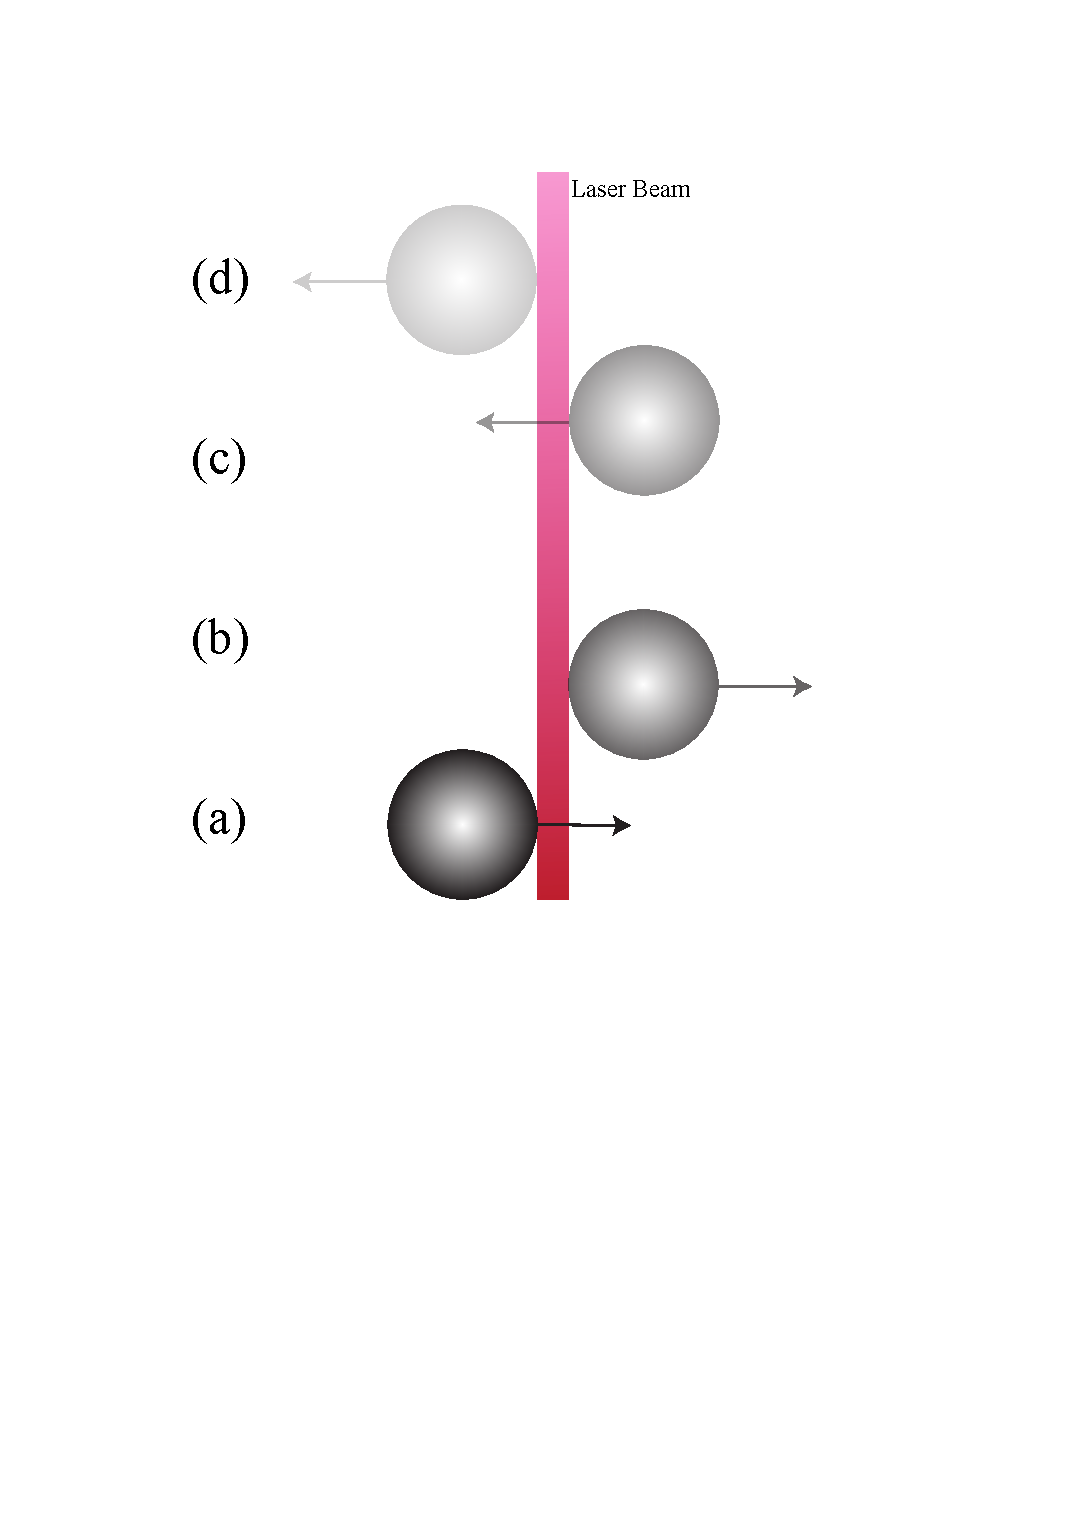
\includegraphics[width=.3\linewidth]{Figures/extractingData/OpticalSwitch.png}%
  \caption{The idea behind an optical switch---each time the pendulum enters or leaves the beam, a digital timing signal is recorded. In the figure, the pendulum is drawn a four different times; on the 5th crossing (not shown), one will have enough information to calculate the period.}
  \label{fig:opticalSwitch}%
\end{figure}

\begin{figure}[htb]
 \includegraphics[width=0.85\linewidth]{Figures/extractingData/Output.png}%
  \caption{A plot (using Matplotlib) of the period vs time data from the full data set. Notice that Matplotlib automatically pulled out 3.462 s from the period axis on the left, so that the vertical tics are space 0.4 ms apart, and over the course of 850 seconds, the period of the pendulum only changed by about 1 mS.}
  \label{fig:Output}%
\end{figure}


\section{Details for this Assignment }\label{sec:task1}
\begin{enumerate}
	\item Read the file {\textsf PeriodData.dat}, and extract only lines with actual period values. Create an output file called {\textsf Filtered.dat} (which will go in your data folder---see Appendix~\ref{app:submission} for submission guidelines). I've posted one way (not the most elegant, but it works) to do this at \href{http://people.usm.maine.edu/pauln/261downloads.html}{http://people.usm.maine.edu/pauln/261downloads.html} in file filter.py
	\item Plot this data from within your script using Matplotlib. I suggest you go to the Matplotlib gallery, find a simple x-y plot similar to what you want, and examine the code needed to create the plot.
	\item Once you create the plot on the screen, you can click the disk icon on the plot to save it to disk (in your \verb&LaTeX/Figures& folder) as a .png or a .pdf file. 
	\item As a part two to this exercise, still using the data from periodData.txt (at \href{http://people.usm.maine.edu/pauln/261downloads.html}{http://people.usm.maine.edu/pauln/261downloads.html}) create a data file with all possible periods extracted; i.e. you can calculate the period as the difference in time between every 4th crossing:
	$$ \mathrm{Period}_i = t_{i+4} - t_i$$
In this scheme, you'll end up with roughly three times as many period measurements. Create a new output file called \textsf{tripleFiltered.dat}, and plot this data file as you did with \textsf{filtered.dat}. Keep in mind that you will have to modify your program to produce this data file. 
	\item Now write a short \LaTeX\ report about what you did. This is \textbf{not}
	a formal report, but simply an exercise to get your Linux/Python/LaTeX feet wet. When you're done, you'll have had experience with the three main tools we'll work with all semester, so the rest of the term will polish and deepen your familiarity with these tools.
	\item Don't forget to submit your completed assignment according to the format specified in Appendix~\ref{app:submission}. Your python scripts for part 1 and part 2 should of course be in your code folder. You do not have to use the code I posted to do part 1---if you have a better way, please feel free to ignore my code, and I'll include a handout of all the different methods people used when I hand back your assignment submissions. 
\end{enumerate}


%%%%%%%%%%%%%%%%%%%% chapter1.tex %%%%%%%%%%%%%%%%%%%%%%%%%%%%%%%%%
%
% sample chapter
%
% Use this file as a template for your own input.
%
\chapter{Python Basics}
\label{basics} % Always give a unique label
% use \chaptermark{}
% to alter or adjust the chapter heading in the running head
\section{General Overview}
\label{sec:overview}
This chapter will assume that you have installed a working version of Python 2.7 on your computer. In order to use Python, you have to type commands, and to do so you have several options. First, your installation of Python likely comes with a Python interpreter (on the Enthought Python installation, it is called IDLE). Double-clicking on this application will start a python shell window. Second, you can open (in Linux or OS X) a terminal window and type
\begin{verbatim}
	python
\end{verbatim}
You will then see something like this:
\small\begin{verbatim}
Enthought Python Distribution -- www.enthought.com
Version: 7.1-2 (64-bit)

Python 2.7.2 |EPD 7.1-2 (64-bit)| (default, Jul 27 2011, 14:50:45) 
[GCC 4.0.1 (Apple Inc. build 5493)] on darwin
Type "packages", "demo" or "enthought" for more information.
>>> 
\end{verbatim}\normalsize
The notation \verb">>>" indicates that Python is ready to accept commands, and is an interactive mode.
These first two options are almost identical in their function, so I'll leave it to the reader to choose which is most convenient.
The third option is to use a text editor to write Python code and then compile the code either with the terminal, or, if the text editor is powerful enough, from within the text editor itself. On OS X, there is an excellent editor called TextMate, which excels at this. In fact, TextMate was also the editor used to write the \LaTeX\ code for this book. A cross platform and open source option is Geany. The last option is to use an integrated development environment; there are many programs in this category, but I opt not to use this route because of the overhead needed, and my bias that a closer contact to the code and compilation is better for understanding what is happening when learning to program.

This textbook will use the interactive mode (through either the terminal or IDLE) and compiling text files containing Python code. For short programs, or for developing code, it is convenient to use the interactive mode, as you can get immediate feedback. More on this soon. For the bulk of our work in this text, we will assume you are using a text editor, and write files which are then run by the Python interpreter. Whenever you see the notation \verb">>>", this is an indication that Python is being used interactively, and it's a good idea to try out the examples. 

This chapter will explore the interactive mode, extending Python with external libraries, how to write and compile Python code, and generally provide you with a baseline of tools needed to get started programming so that we can get to the physics as quickly as possible. 

\section{Python as an Interactive Calculator}
\label{sec:calculator}
% Always give a unique label
% and use \ref{<label>} for cross-references
% and \cite{<label>} for bibliographic references
% use \sectionmark{}
% to alter or adjust the section heading in the running head
One of the wonderful features of Python is the ability to use it in an interactive fashion, and also, the simplicity of its syntax. For example, suppose you want to perform a simple calculation such as adding two numbers. Open up a terminal window type \texttt{python} and type \texttt{print 2+5}; you will see the following:
\small\begin{verbatim}
	>>> 2+5
	7
	>>> 
\end{verbatim}\normalsize
Python simply prints the result of the operation, and the interpreter shows a new prompt indicating it is ready for further input. Notice that we simply have added two integers without having to declare them as such. Python makes an intelligent decision based on whether we input integers or floating point numbers; it assumes that if you do not enter a decimal point, that the number is an integer, and otherwise (with the exception of complex numbers) the number is a floating point (called a \verb2float2 in Python parlance). Notice that we have to be careful when dividing as the following examples show (comments are mine):
\small\begin{verbatim}
	>>> 2/5	  # dividing two integers gives the lowest integer
	0
	>>> 5/2	  # same thing here.		
	2
	>>> 5./2   # here we divide a floating point number by an integer
	2.5
	>>> 5/2.   # same here
	2.5
\end{verbatim}\normalsize
Notice that we can put a comment within a line of Python input. A \# sign starts a comment; anything after this character is ignored.

In physics, we often have more complicated arithmetic, such as the expression $\pi\times 10^{7} \cdot \sqrt{90.1}$. This is accomplished as follows: 
\small\begin{verbatim}
	>>> from math import *
	>>> pi*10**7*sqrt(90.1)
	298203178.477 049 65
\end{verbatim}\normalsize
In order to use the value of $\pi$, we have to first load the math library; the statement \texttt{from math import *} loads all of the functions from the math library, including trigometric and logarithmic functions. This will be a standard library to include in most of the Python programs in this book. 
Also notice that Python understands the order of operations, and we did not need parenthesis. The calculation we performed here involves both integers and floating point (i.e. numbers with decimal points) numbers. 

Now, if you are being a skeptical student, you will have checked the previous calculation with your calculator, and verified that it appears to agree (actually, your calculator will likely only give you an answer to the 4th decimal place). However, if you perform the calculation in Mathematica 6.0, and C++, you will find that the answers are 
\small\begin{verbatim}
	298,203,178.477 049 591 064 453 125		(Mathematica 6.0)
	298 203 178.477 049 589 157 104 492 	(C++, gnu compiler)	
\end{verbatim}\normalsize
Notice that these disagree with the Python calculation in the 16th significant digit. In this case, I would likely trust the Mathematica result, as it is specifically designed for high precision calculations. However, the point here, is that Python (and C++, Fortran, etc) have inherent numerical limitations (typically about 16 digits of accuracy for double precision floating point numbers). We have to be careful to not perform calculations where this limitation is significant.

\section{Python libraries: Loading and getting help}
\label{sec:mathlibrary}
As we have already seen, the core of the Python language is easily extensible by loading libraries (most of which are freely available) There are libraries for mathematics, graphing functions, 3d visualization, and many others. Here, we look a little more closely at the math library and how to find out about the available functions. 
%
% For tables use
%
\begin{table}
\centering
\caption{A partial list of constants and functions in the Python math library.}
\label{tab:mathlibrary}       % Give a unique label
\begin{tabular}{ll}
\hline\noalign{\smallskip}
Function\hspace*{7mm} & Description  \\
\noalign{\smallskip}\hline\noalign{\smallskip}
sqrt(x) 		&	Returns the square root of x\\
exp(x)		&	Returns $\exp(x)$ \\
log(x)		&	Returns the natural log, i.e. $\ln(x)$\\
log10(x)	&	Returns the log to the base 10 of x \\
degrees(x)	&	converts angle x from radians to degrees\\
radians(x) 	&	converts angle x from degrees to radians\\
pow(x,y)	&	Return $x^y$; you can also use x**y  \\
hypot(x,y)	&	Return the Euclidean distance, $\sqrt{x^2 + y^2}$\\
sin(x)		&	Returns the sine of x\\
cos(x)		&	Return the cosine of x\\
tan(x)		&	Returns the tangent of x\\
asin(x)		&	Return the arc sine of x\\
acos(x)		&	Return the arc cosine of x\\
atan(x)		&	Return the arc tangent of x\\
atan2()		&   Return the arc tangent of y/x.\\
fabs()		&   Return the absolute value, i.e. the modulus, of x\\
floor()		&   Rounds a floating point number down\\
ceil()		&	Rounds a floating point number up\\
\noalign{\smallskip}\hline\noalign{\smallskip}
Constant 	& 	Description  \\
\noalign{\smallskip}\hline\noalign{\smallskip}
e			& 	$e=2.718...$\\
pi			&	$\pi=3.14159...$\\
\noalign{\smallskip}\hline
\end{tabular}
\end{table}
%

Table~\ref{tab:mathlibrary} lists some of the functions available in the Python math library; in addition, one can always get complete information about the functions available in a given library by using the \verb2help()2 command:\small
\begin{verbatim}
	>>> import math
	>>> help(math)
\end{verbatim}
\normalsize

I haven't printed the output of the help command here to save space, but you should get familiar with this command, as it is a useful feature of Python that applies to other libraries too. Also notice that in order to get help on the elements of a library, one has to import the library (in this case \verb2import math2) in a different manner than we used in to actually access the functions within the library. 

\subsection{Two methods of loading libraries}
\label{sec:LoadingLibraries}
When importing libraries into Python, we have two alternatives (math library used as an example):
\begin{enumerate}
	\item \lstinline2from math import *2
	\item \lstinline2import math2
\end{enumerate}
This text will usually use method (1) which loads all of the functions in the math library. The advantage of this method is that it allows us to call a function by its name in the particular library, for example, to calculate the sine of x, we simply type 
\begin{verbatim}
	sin(x)
\end{verbatim} 

Method (2) also loads the entire math library, but now to calculate the sine of x, we must type
\begin{verbatim}
	math.sin(x)
\end{verbatim}
This method, although it involves more typing, has the advantage of explicitly addressing the function sin() contained in the math library. For instance, you could also have your own function defined (more on functions soon) which was also called sin() and there would be no conflict between the two. Of course, it would be bad programming practice to define your own function with the same name as a known function in the math library, but if it was important to do so, this alternate method of loading the library would allow it. 


However, in order to be able so get help on the contents of the library, we must import the library itself. This is outlined in section~\ref{sec:mathlibrary}. \\
(a) Start a python session using a terminal window or using IDLE. Import the math library and type \verb2help(math)2 as outlined in section~\ref{sec:mathlibrary}. (Do not type \lstinline2from math import *2) If you are using a terminal window (as opposed to IDLE) you need to know the following: the space bar goes to the next page, and the \verb2q2 key exits. Read about the hypot(x,y) command. \\
(b) Now, to evaluate \verb2hypot(3,4)2, you will have to type \verb2math.hypot(3,4)2. Try it and verify that you get the correct answer.\\
So, what's the point of this method of importing the math library? It insures that when you want to use a function specific to that library, you have to expressly indicate so; if we type \lstinline2>>>from math import *2, we have the advantage of being able to address the functions without the \verb2math.func()2 notation, but we run the risk (in a sufficiently complicated program) of defining our own function with the same name. Then, we could get unexpected results. A sufficiently cautious programmer would, I suppose, opt to use the safer \lstinline2import math2 style. Another reason that it is sometimes preferable to use this method, is that it explicitly indicates which library the function is from, which aids in understanding the program or finding documentation (if you import with the * notation, you lose the ability to know which library the function belongs to). This book will mix the two methods, but you are free to use either method in your code.


Problem~\ref{prob1.2} will give you some more experience with using help(math)
as well as exploring some of the functions in the math library.
For a partial list of functions in the math library, see Table~\ref{tab:mathlibrary}. 


\subsubsection{Other Libraries}
\label{sec:OtherLibraries}

There are several Python libraries that we will use in this text; however,  since my goal is to get us thinking about physics as soon as possible, I will discuss their usage as we go. For complete documentation on the Python language, see the  \href{http://docs.python.org/}{Python Library Reference}. Click on the \href{http://docs.python.org/lib/module-sys.html}{Library Reference} link to see full documentation on each library. 

\subsubsection{Alternate Help via pydoc}
\label{sec:pydoc}
Another way to get help---not within a Python session, but on the command line (i.e. a terminal window)---is with \verb!pydoc!, which is included with Python. Typing \verb!pydoc Z!, where \verb!Z! is any function or module within Python's path, will reveal documentation on that item. For example, opening a terminal window and typing \verb!pydoc math.sin!
will reveal documentation on the sine function. 



\section{First Python Program}
\label{sec:FirstProgram}

Let's get started by writing our first Python program that, while not terribly useful, illustrates how to read input and write output to and from the screen. Typically, this is called a ``hello world'' program, but we'll make it a little more interesting by having if actually do something a little more complicated. 

Our first program will simply calculate the vertical position of a ball thrown vertically upward from the surface of Earth at a time $t$ after launch. For simplicity, we make the standard assumptions of constant acceleration due to gravity and no air resistance.
The physics of this motion is simple. The ball's vertical position is given by 
	\begin{equation}
		y(t) = v_0 t - \frac{1}{2}gt^2 .
	\end{equation}
Each program should be proceeded by an outline (or in more complicated programs, a full--blown flowchart illustrating all of the logical steps) that lays out the steps needed. Here is a simple outline for our program:
\begin{enumerate}
	\item Read input velocity, $v_0$ and the time $t$
	\item Compute the position at time $t$
	\item Print out the result
\end{enumerate}
 Here is the Python code needed: \\
\lstinputlisting[
caption={Our First Python Program},
label=FirstProgram, 
style = myPythonStyle]
{Code/4BasicPython/program1.py}

To create a python program with this code, it is helpful to use a Python aware text editor, so that the editor will perform syntax highlighting and formatting specific to Python. On the Mac, I recommend TextMate (shareware) or Smultron, Vi, or Emacs (open source). Another option (which is also cross platform and open source) Having chosen a suitable editor, create a new file and give it a .py extension, or download the file program1.py from the \href{http://www.usm.maine.edu/~pauln/CompPhysPython}{text website}. Decide where you are going to keep your programs, and start off by thinking about a logical scheme. I suggest you create a folder called MyPrograms and place it in your home user folder. Then, since you will likely have many programs in here, it makes sense to have each program in its own subfolder, so that any files or images generated stay organized and associated with the original Python program.

To run the program, open a terminal window (on the Mac, this is in the Applications/Utilities/ folder). Then, before running the program, you have to change your directory (unix command=cd) to your current program folder. To do this, you have two options on the Macintosh: 
\begin{enumerate}
	\item With the terminal window open, type \verb2cd MyPrograms/Program1/2
	followed by the RETURN key. 
	\item With the terminal open, type \verb2cd 2 (with a space after cd) and then drag the folder Program1 (or whatever you have called it) to the terminal window. The Mac OS will copy the address of the folder to the terminal. Then click on the terminal window and press RETURN.
\end{enumerate}
To run the program with an initial upward velocity of 19.6 m/s and a time 3.0 seconds, type
\begin{verbatim}
	python program1.py 19.6 3.0
\end{verbatim}
followed by RETURN.
Python returns the answer of 14.7 meters, as seen in Figure~\ref{fig:FirstPythonProgram}.
\begin{figure}
\centering
\includegraphics[height=7cm]{Figures/4BasicPython/TerminalWindow1}
\caption{Running our first Python program}
\label{fig:FirstPythonProgram}       % Give a unique label
\end{figure}

\subsection{Discussion of Code}
\label{sec:Program1Discussion}
The first line imports the \lstinline2sys2 (system) library, and which we use in this program to be able to pass input values for the initial velocity and the time to the program. The second line imports all the functions of the math library (which, in this case we don't need, but I include anyway since most programs will need the math library). 

The next section is a \lstinline2try...except:2 block specific to Python which is the standard method for dealing with potential errors. The system library contains a text array called \lstinline2argv[]2; sys.argv[0] contains the name of the python program (sometimes called a script instead), sys.argv[1] and sys.argv[2] refer to other parameters passed to the program (in our case, v0 and t). When Python encounters a \lstinline2try...except2 block, it attempts to execute the elements in the \lstinline2try:2 block, and, if successful, passes control to what follows the \lstinline2except:2 block. 

So, in our case, the program reads the three parameters that you entered when running the program in the terminal: sys.argv[0] is the name of the program (in this case program1.py), sys.argv[1] is defined to be v0, and sys.argv[2] is defined to be t. If an error occurs---for instance, you forget to enter any values for v0 and t when you call the program---then the \lstinline2except:2 block is executed. 

In the case of an error the \lstinline2except:2 block prints out a reminder to the user to call the program with two arguments (v0 and t), and then calls another system routine which exits the program. 

The last portion of the program is only executed when there are no errors, and that consists of a straightforward calculation of the height of the projectile and a simple print statement. In Python, it is acceptable to use either single or double quotes; this example uses double quotes.

Although this first program is very simple, the \lstinline!try:...except:! block is a significant chunk of the script, and the program could be made considerably shorter without it; the script would then be written simply as
\begin{lstlisting}[frame=none, style = pythonSnippet]
	import sys
	from math import *

	v0 = 19.6 		# initial velocity
	t = 3.0			# time			
	y = v0*t-4.9*t**2	#  position 
	print "ball's position is", y, "meters at t=", t, "seconds"
\end{lstlisting}
In this case, the code is clearly more readable, but now, to run the script with different values for the initial velocity and time, the code would have to be edited and saved, and then you would have to execute the script from the terminal once again. Reading the input parameters from the command line using  the  \lstinline!try:...except:! block gives one the ability to re-run the code without going through this extra step. 

Two other comments about Python that we will encounter as we move forward: in Python, we do not have to end lines with semicolons (as in C and C++), and do not have to use braces to demarcate the extent of structured environments. For instance, in this example, the extent of the \lstinline2try2 and of the \lstinline2except:2 blocks are completely demarcated by the indentation. So, it is critical to be very careful with indentation in Python. It makes for very easy to read code, but forces the programmer to be mindful of indentation when coding. The second comment is that you should get in the habit of using comments to explain your code and make it readable to other users (and yourself). Comments in Python are preceded by a \# sign; anything on the line after this character is ignored. Commenting your code achieves several things; it makes you explain your code (which often catches errors in reasoning), and it makes your code easier to decipher, especially when others may not understand your choice of variables. 

\section{Second Python Program}
\label{sec:SecondProgram}

Now that we have written a simple Python program, we are ready to add more to our toolbag. Lets see how to incorporate graphics into our output; we'll modify our program to plot the vertical position of the ball as a function of time. In doing so, we will also learn about loop structures, reading and writing data to files, and the MatplotLib plotting library. Here is the Python script that accomplishes this. 

\lstinputlisting[caption={Our second Python program adds graphical output using MatPlotLib.}, label={SecondProgram}]{Code/4BasicPython/program2.py}

\subsection{Running the script}
\label{subsec:running}

Once you've created a file with the above code, save the file as \verb!program2.py! and then open a terminal window. Change your directory to the folder containing your script; let's assume you place the script in a folder \verb!Program2! which is a subfolder of the \verb2MyPrograms2 folder in your home directory. Then type
\begin{verbatim}
	cd MyPrograms/Program2/
\end{verbatim}
and then, assuming that you want to create a data file called \verb2trajectory.dat2, and you want to launch the ball upward at 19.6 m/s, plot the vertical position for 4 seconds, and plot points every 0.1 seconds, you would type 
\begin{verbatim}
	python program2.py 'trajectory.dat' 19.6 4.0 0.1
\end{verbatim}
Python will create the data file, and display the graphic shown in 
Figure~\ref{fig:SecondPythonProgram}. 
\begin{figure}
\centering
\includegraphics[height=8cm]{Figures/4BasicPython/trajectory.pdf}
\caption{MatplotLib output from our second Python script. Clicking the bottom rightmost disk icon at the bottom of the plot will save the figure as a .png file. To return control to the terminal, simply close the window. Explore the other buttons to see some of the interactive features provided with every Matplotlib figure.}
\label{fig:SecondPythonProgram}       % Give a unique label
\end{figure}

\subsection{Discussion of the Script}
\label{subsec:DiscussionOfScript}

Our second Python script starts by an extended comment (the triple quotes demarcate a special comment called a docstring, which is useful in documenting this piece of Python code. More on this in a later chapter. Then the script procedes by loading the libraries we will need. The system (sys) library for reading and writing data, and the pylab library for accessing Matplotlib, which is a Matlab-like plotting library. The distinction between pylab and Matplotlib is actually a bit unclear to this author, as even the Matplotlib web site presents the two packages as synonymous, however, it will not work in this case to replace \verb!from pylab import *! with \verb!from matplotlib import *!. 

The next block of code uses a  \lstinline!try:...except:! block to read in the output file name, the initial velocity, the length of time to follow the ball, and the time step. 

After reading in these parameters from the terminal, we define \verb2outfile2 to open an output file to write data to:
\begin{verbatim}
	outfile = open(outfilename, 'w')
\end{verbatim}
where \verb2open2 is a system library function that opens creates the file, and \verb2outfile2 is an arbitrary user create variable. If there is a need to write multiple output files, then one must create a variable to point to each file. The \verb2'w'2 indicates that the file is prepared for being written to; if we wanted to open a file for reading, we would use \verb2'r'2 instead of \verb2'w'2. We then define the acceleration due to gravity, and set the start time to 0 seconds. 

Now, we introduce a new structure called a function. We define a function called \verb2height(v0,t)2 which has two inputs, the initial velocity, and the time. Within this function, we have a decision structure called an \verb2if...else2 statement. In our example, if the initial velocity is greater than zero, then the function \verb2height(v0,t)  returns2 the height of the ball at time t using the standard kinematic result. If the ball's initial velocity is less than or equal to zero, then a statement to this effect is printed to the terminal, and the program exits. 

Notice that the extent of the body of the function is demarcated by the indentation; the blank line after \verb2sys.exit(1)2 is purely for a visual readability of the code. In addition, indentation also governs the extent of the \verb2if...else2 statement. Note that Python executes code sequentially, so that the function \verb2height()2 must be defined \textit{before} it is used; for example, it won't do to place this function at the end of the script---Python will give an error if this occurs. 

The next line writes the column labels, \verb2time (s)2 and \verb2height (m)2, as the first line of \verb2outfile2. Between these column headings is a tab character, represented as \verb2\t2, and at the end is a newline character, \verb2\n2. 

The physics in this program is in the main calculation loop. First I calculate the number of steps needed to iterate over given a time of \verb!tmax! and a time step of \verb!dt!.

The main calculation is a loop that uses a \verb2for2 statement. This statement tests a condition, and if true, executes the body of the loop (demarcated by indentation, of course). In our case, we use Python's \verb2range()2 function, which has three possible forms:
\begin{enumerate}
	\item range(n) : returns a list of integers from 0 to n-1 
	\item range(a,b): returns a list of integers from a to b-1
	\item range(a,b,dn): returns a list of integers from a to (b-dn) in incements of dn.
\end{enumerate}
For example: 
\begin{verbatim}
	>>> range(3)
	[0, 1, 2]
	>>> range(1,3)
	[1, 2]
	>>> range(1,10,2)
	[1, 3, 5, 7, 9]
\end{verbatim}
So, the \verb2for2 statement starts with i=0, evaluates the next three lines, then reads the next value of i, executes the three lines again, reads the next value of i, etc. 
Execution of the loop ceases after evaluating the loop for the i=imax-1, then the output file is closed. So, in our code, in order to plot points from \verb!t=0! to \verb!t=tmax!, we must have our for statement read
\begin{lstlisting}[frame=none]
	for i in range(imax+1)
\end{lstlisting}
otherwise, we will end up one time step short of the maximum. This (at least to me) is a slight annoyance of Python (an C/C++ too), but we are stuck with this fact that indexing starts from zero in Python. The rest of the \verb!for! loop calculates the time, the height (using our defined function \verb!height()!), and then writes out the time and height to our output data file, one line at a time. Notice that the write statement
\begin{lstlisting}[frame=none]
	outfile.write('%g \t %g\n' % (t,y))
\end{lstlisting}
consists of two pieces. The first 
\begin{verbatim}
	'%g \t %g\n'
\end{verbatim}
is called a format string, and it defines that two numbers are to be written to the output file. The first number is a floating point (\verb!%g!), followed by a tab character (\verb!\t!), another floating point number, and finally, a newline character (\verb!\n!). This format string is inherited from the C programming language; at its most basic level, a format string has the form
\begin{verbatim}
	%<width>.<precision><type-character>
\end{verbatim}
where the width and precision are optional arguments, and not all formats (shown in Table~\ref{tab:FormatSpecifiers}) can accept width and precision arguments. For example, if x=1234.5678 the format string 
\begin{verbatim}
	%10.4f
\end{verbatim}
indicates that a floating point number with 10 digits will be written with 4 decimal places shown. Since x has 9 characters (the decimal point counts as one character), the above print statement will pad the output with one blank space at the left. On the other hand, the \verb!%g! format is a \textit{general} format specifier that defaults to a precision (read:\# significant figures) of 6. To specify the number of significant figures with the \verb!%g! format, the width argument is irrelevant, and the precision argument specifies the number of significant figures. So, if x=1234.5678, a Python terminal session will produce the following:
\begin{verbatim}
	>>>print '%10.4f \n' % x 
	 1234.5678				# note the space at the left
	>>>print '%9.4f \n' % x 
	1234.5678
	>>>print '%g \n' % x 		# %g defaults to 6 signif. figs
	1234.567
	>>>print '%.6g \n' % x 		# same as default!
	1234.567
	>>>print '%.7g \n' % x 		
	1234.568
	>>>print '%.8g \n' % x 		# now the full number is shown
	1234.5678
	>>>print '%.8f \n' % x 		# this will show 8 decimal places
	1234.56780000				
\end{verbatim}

If you ever want to see the result of a particular formatting statement, you can always see the results in an interactive terminal session---one of the benefits of Python over compiled languages. For reference,  Table~\ref{tab:FormatSpecifiers} shows a list of common format specifiers.
\begin{table}
\centering
\caption{A partial list of format specifiers in Python. For more information, see the \href{http://docs.python.org/}{Python Documentation}, click on Library
Reference, and search for \href{http://docs.python.org/lib/typesseq-strings.html}{String Formatting Operations}. }
\label{tab:FormatSpecifiers}       % Give a unique label
\begin{tabular}{ll}
\hline\noalign{\smallskip}
Specifier\hspace*{7mm} & Description  \\
\noalign{\smallskip}\hline\noalign{\smallskip}
d&	Signed integer decimal.	\\
i&	Signed integer decimal.	\\
o&	Unsigned octal.\\
u&	Unsigned decimal.\\	
x&	Unsigned hexadecimal (lowercase).\\
X&	Unsigned hexadecimal (uppercase).\\
e&	Floating point exponential format \\
E&  Same as \verb!%e! except an upper case E is used for exponent.\\
f&	Floating point decimal format.\\
g&	Floating point format. Uses exponential format if exponent is\\
 & greater than -4 or less than precision, decimal format otherwise.\\
G&  Same as \verb!%g! except an upper case E is used for the exponent.\\
c&	Single character (accepts integer or single character string).	\\
r&	String (converts any python object using repr()).	\\
s&	String (converts any python object using str()).\\
\noalign{\smallskip}\hline
\end{tabular}
\end{table}
%

The last portion of the program uses pylab/matplotlib to read the data and plot it to a new window on the computer The \verb!load! command is from the pylab library; remember, you can get help on this command by opening a terminal window, and typing 
\begin{verbatim}
$ python
>>> import python
>>> help(pylab.load) .
\end{verbatim}
The lines
\begin{lstlisting}[frame=none]
xaxis = data[ : , 0 ]			# first column
yaxis = data[ : , 1 ]			# second column
\end{lstlisting}
define two lists \verb!xaxis! and \verb!yaxis! to be the first and second columns of the array \verb!data!. Note that because python starts arrays with index zero, the first column is column 0. The remaining commands use \verb!Matplotlib! to plot these two lists. Notice that the plot produced comes with a toolbar along the bottom of the display. Your should experiment with them to see what options they present (one of them is to save a copy of the plot to disk). To exit the plot and return control to the terminal, you have to close the window. 

There are many more features of Matplotlib; if you are eager to see more, you can see the \verb!Matplotlib! \href{http://matplotlib.sourceforge.net/tutorial.html}{tutorial}, and for a complete reference, see the \href{http://matplotlib.sourceforge.net/}{User's Guide} at the \verb!Matplotlib! home page. We will learn to use other features of this plotting library as we progress forward. 

\section{Saving Functions as Modules}
\label{sec:Modules}
Although our second program (~\ref{SecondProgram}) is not terribly complicated, as we develop more involved codes, it is good practice to modularize our code. There are two primary ways to accomplish this; one is to use the object--oriented features of Python and another is to split off functions into separate pieces of Python code called \href{http://docs.python.org/tut/node8.html}{modules}. For example, we can split the function \verb!height(vo,t)! from our main script, and save it as a separate file; however, it is a good idea to make a small change to the \verb!height! routine by adding an option for the acceleration due to gravity, with g=9.8 m/s$^2$ being a default value. Here is the modified \verb!height()! routine, saved as \verb!analytic.py! (named both to remind us that this is the analytic solution for the height, and to avoid an awkward function call):
%
\lstinputlisting[caption={Sections of code can be saved as reusable functions}, label=snippet]{Code/4BasicPython/analytic.py}
% 
If we wanted to call the height function from our main program, we have to make sure to place \verb!analytic.py! in the same folder as \verb!program2.py!, and make sure to import it either by \\
\verb!import analytic!\\
or \\
\verb!from analytic import height! (or \verb!from analytic import *!).\\
Then, to call the function, we have to use either analytic.height(v0,t), or height(v0,t), respectively. Notice that due to the inclusion of g=9.8 in the definition of the function, we do not need to pass the acceleration due to gravity; however, if we wanted to, we could alter the value of g in the function call by, for instance, \verb!height(v0,t,g=4.9)!. 
Here is the code of Listing~\ref{SecondProgram} modified to use our function \verb!height()! which is included in the file \verb!analytic.py!:
%
\lstinputlisting[caption={Our first program made modular.}, label=ThirdProgram]{Code/4BasicPython/program2_mod.py}
%


\section{Other Data Types in Python}
\label{sec-datatypes}
Although we will primarily be using floating point numbers and integers, Python also has several other data types that we will use: Boolean, complex numbers, strings, and lists. 
\subsection{Boolean Integers}
\label{subsec-boolean}
A boolean variable in Python is actually an integer; either False (0) or True (1), which you can see if you attempt to use them as in a numerical context. The following examples illustrate the use of booleans: 
\begin{verbatim}
	>>> b=1<2 
	>>> b
	True
	>>> b+1
	2
	>>> bool(b)
	True
	>>> bool(20<100)
	True
	>>> bool(20<=19)
	False
	>>> bool(20<=20)
	True
\end{verbatim}
\subsection{Complex Numbers	}
\label{subsec-complex}
Complex numbers in Python are created by one of two methods: 
\begin{lstlisting}[frame=none]
a=1.0 + 2.0j 	# you can also use uppercase J if you like
a=complex(1,2)
\end{lstlisting}
and the real and imaginary parts are represented internally as floating point numbers (even if you type them without a decimal point). You can extract the real and imaginary parts and obtain the modulus  as follows:
\begin{lstlisting}[frame=none]
>>> z=3 + 4j 
>>> z.real
3.0
>>> z.imag
4.0
>>> abs(z)
5.0
\end{lstlisting}

\subsection{Strings}
\label{subsec-strings}
Strings are simply sequences of alphanumeric characters, and in Python, can be enclosed in single or double quotes. You can also refer to a specific character by its position in the sequence, and can also easily extract a range of characters:
\begin{lstlisting}[frame=none]
>>> x='Ministry of Silly Walks'
>>> x
'Ministry of Silly Walks'
>>> x[0]
'M'
>>> x[5]
't'
>>> x[0:8]
'Ministry'
\end{lstlisting}
You can also add a character to a string in a straightforward manner:
\begin{lstlisting}[frame=none]
>>> y=x+'!!'	# creates a new string with added exclamation points
>>> y
'Ministry of Silly Walks!!'
>>> z=y[ :-2]	# creates a new string which is every character from
>>> z		# y except the last two characters.
'Ministry of Silly Walks'
\end{lstlisting}
Being able to add a character(s) to a string is especially convenient when writing a series of output files with slightly different names. 

\subsection{Lists}
\label{subsec-lists}
A list is a compound data type composed of several comma-separated values enclosed by square braces; the individual elements need not be of the same data type:
\begin{lstlisting}[frame=none]
>>> misc=['silly', 8, 2.0, 3.0 + 4.0j]
>>> misc[0]		# extracts first element of misc
'silly'
>>> misc[1]*misc[2]	# you can multiply elements together if appropriate
16.0
>>> misc[1]*misc[3]	# even this is okay
(24+32j)
>>> misc[-1]	# displays last element
(3+4j)
>>> new=misc + ['walk', 3.14]	# create new list 
>>> new
['silly', 8, 2.0, (3+4j), 'walk', 3.1400000000000001]
>>> len(new)	# the number of elements in the list
4
\end{lstlisting}
There are many other features of lists, and we will introduce them as needed.


\section{Flow Control: if, while, for}
\label{sec-flow}
There are three main ways to control the flow of program execution in Python. We will look briefly at each. 

\subsection{if Statements}
\label{subsec-if}
The if-statement has the general form 
\begin{lstlisting}[frame=none]
	if <expression is true> :
		then execute
		each indented line
	otherwise continue on to next unindented line
\end{lstlisting}
Here is a simple example:
\begin{lstlisting}[frame=none]
i=10
if i <= 100:	# note colon at end of line
	i=i+1
print i
\end{lstlisting}
Running the above will print out a result of 11 for i. 

Often, a single \verb!if! statement is not sufficient, so Python provides for \verb!if!\ldots \verb!else!
 and \verb!if!\ldots \verb!elif!\ldots \verb!elif! \ldots structures. The \verb!else! portion is optional, and \verb!elif! is short for \verb!else if!. The logic is fairly straightforward, as this simple example shows: 
\begin{lstlisting}[frame=none]
i=100	#note that one equals sign assigns the value 100 to i.
if i < 100:
	print 'i<100'
elif i==100:	#note that two equals signs are needed to test for equality
	print 'i=100'
elif i>100:
	print 'i>100'
else:
	print 'it is not possible to get here!'	
\end{lstlisting}

\subsection{while Statements}
\label{subsec-while}
\verb!while! statements are used to iterate over a range of values. The extent of the loop is controlled by indentation, and the loop executes repeatedly until the condition is no longer true. \verb!while! loops have the general format
\begin{lstlisting}[frame=none]
	while <expression is true> :
		execute each indented line
		return to the beginning
		of the while loop to retest 
		the condition. When the test fails,
	exit the loop to the next un-indented line
\end{lstlisting}
Here is a simple example that sums the integers from 0 to 100:
\begin{lstlisting}[frame=none]
	i,sum =0,0	# we can assign values to i and sum simultaneously
	while i<=100:
		sum=sum+i
		i=i+1		
	print sum
\end{lstlisting}
This code properly prints out the sum as 5050, which is obviously correct, since there are 50 sets of 101 (1+100, 2+99, 3+98, \ldots). 

\subsection{for Statements}
\label{subsec-for}
The \verb!for! statement in Python iterates over all of the items in a sequence (which can be a list of numerical values, or even a list of string variables). Typically, for numerical programming, we will make use of the \verb!range()! function as discussed in Section~\ref{subsec:DiscussionOfScript}. Here is an example that sums the integers from 0 to 100 using a \verb!for! statement:
\begin{lstlisting}[frame=none]
	i,sum =0,0	
	for i in range(101):	# note that range(101) consists
		sum=sum+i	# of integers from 0 to 100
		i=i+1		
	print sum
\end{lstlisting}



\section{General Guidelines for Programming}
\label{sec-programmingGuidelines}
Writing a Python script or program is necessarily an individualistic endeavor; those of you just learning the language will clearly write different programs than those who have previous experience. However, There are several guidelines that are good to follow: 
\begin{itemize}
	\item Start each program with a pen and paper outline of its structure. For simple programs, this can be a short bit of pseudo code (just a brief outline of the logical steps the script needs to accomplish); for more complicated programs, you will need to actually create a flowchart that explicitly outlines the many logical steps needed. 
	\item When it comes to writing code, get in the habit of using a logical format; here is a structure suggested by Wesley J. Chun in his book \textit{Core Python Programming}\cite{chun2007}:
	\begin{enumerate}
		\item Startup line (Unix; \verb2#!/usr/bin/env python2)
		\item module documentation (this is what appears between the triple quotes)
		\item module imports (import statements)
		\item variable declarations 
		\item class declarations (we'll get to this later)
		\item function declarations 
		\item main body of program
	\end{enumerate}
	
	\item Comment your code as you write. Ideally, your comments should be sufficient for someone else (assumed to be proficient in Python) to understand your code. 
	
	\item Strive for clarity in your code. Especially as you are first learning to program, there is a temptation to include fancy programming techniques. \textbf{Don't}. After you are sure your code produces reasonable results (see the next item!), then you can (if it is worth the time and effort) optimize your code for speed and add new features. 
	
	\item Always be skeptical of your program's output and check it by testing it for trivial cases where you know an analytical result. For instance, in our second program, even though we were simply computing a known analytic solution for a vertically launched projectile, notice the values I input were an initial velocity of 19.6 m/s and a run time of 4.0 seconds; a quick calculation reveals that the ball should hit the ground at t=4 seconds, and this is reflected in Figure~\ref{fig:SecondPythonProgram}. Checking your program's validity is one of the most important steps in computational physics and a considerable effort should be made to insure that it is working properly before you move on to apply the code to regions that do not admit of analytical results. 
	
	\item Modularize your code and/or use object oriented programming when possible. Modularization improves your code's clarity as well as providing code that can be used by other programs. As we have seen, separating off functions into modules is very easy in Python. Object oriented programming is also easy to implement in Python, but we leave this to a later chapter. \marginpar{What chapter?}	

\end{itemize}

\section{Python References}
\label{sec-references}
For Python, I recommend that everyone have a copy of Guido van Rossum's book\cite{guido-introduction} \href{http://www.network-theory.co.uk/docs/pytut/}{An Introduction to Python} handy; this book is available for purchase as a standard paperback, a downloadable pdf file, or is available for reading online. Many more details about Python are clearly covered in his introduction. Guido is the author of the Python language, and is its BDFL (Benevolent Dictator for Life). If you need more detail, see his complete documentation for Python at the \href{http://www.python.org/doc/}{Python web site}. Keep in mind that although I have only discussed the very basics of the language, Python is a very rich programming language, and if there is something you wish you could do, it's probably possible. 

Two other introductory books can are by John Zelle\cite{zelle} and an excellent introduction and reference by Wesley Chun\cite{chun2007}. At a more advanced level, but very geared toward computational physics is Hans Petter Langtangen's \textit{Python Scripting for Computational Science}\cite{langtangen-3ed}. At the writing of this book, the book is was in its second edition, with a third edition underway. Highly recommended.


\pagebreak
%
%
% Problems or Exercises should be sorted chapterwise
\section*{Problems and Tutorials}
\addcontentsline{toc}{section}{Problems}
%
% Use the following environment.
% Don't forget to label each problem;
% the label is needed for the solutions' environment
\begin{prob}
\label{prob1.1}

\textbf{Interactive Python}\\
Use Python interactively to evaluate the following mathematical expressions, and compare to what you would calculate exactly by paper and pencil:\\
(a) $7.5 + \frac{5}{2}$ \hfill (b) $2.0*(3.0\times 10^8)^2$\hfill (c) $tan(\frac{\pi}{4})$ \hfill (d) $3\times 10^{-7}\log (1000)$\\
(e) $\sin(90^o)$\hfill (f) $\cos(\frac{\pi}{2})$\hfill (g) $\ln(e)$\\

\end{prob}

\begin{prob}
\label{prob1.2}
\textbf{Using Python Help}\\
When importing libraries into Python, we will generally use the method described in section~\ref{sec:calculator}. The advantage of this method is that it allows us to call a function by its name in the particular library, for example, to calculate the sine of x, we simply type \lstinline2sin(x)2. However, in order to be able so get help on the contents of the library, we must import the library itself. This is outlined in section~\ref{sec:mathlibrary}. \\
(a) Start a python session using a terminal window or using IDLE. Import the math library and type \lstinline2help(math)2 as outlined in section~\ref{sec:mathlibrary}. (Do not type \lstinline2from math import *2) If you are using a terminal window (as opposed to IDLE) you need to know the following: the space bar goes to the next page, and the \lstinline2q2 key exits. Read about the hypot(x,y) command. \\
(b) Now, to evaluate \lstinline2hypot(3,4)2, you will have to type \lstinline2math.hypot(3,4)2. Try it and verify that you get the correct answer.\\
(c) Read about the atan2() function using help. Evaluate the arc tangent of a vector with x and y components of -2 and +3 respectively. Why is this a useful function (compared to atan()?)

\end{prob}

\begin{prob}
\label{prob1.3}
\textbf{Matplotlib}\\
Write a simple Python program to make a plot of $\cos(2\pi t)$ from t=0 to t=$4\pi$. Hint: look at the \href{http://matplotlib.sourceforge.net/}{Matplotlib web page} and see the \href{http://matplotlib.sourceforge.net/screenshots.html}{screenshots} link for examples complete with code.
\end{prob}

\begin{prob}
\label{prob1.4}
\textbf{Practice with loops, writing to a file, and Matplotlib}\\
(a) Write a simple Python program to print out the Fibonacci series up to some specified maximum integer, N. \\
(b) Now alter the program so that the maximum number N is read from the command line and the Fibonacci numbers are printed out to a file and plotted with Matplotlib. 

\end{prob}

%

%%%%%%%%%%%%%%%%%%%% chapter2.tex %%%%%%%%%%%%%%%%%%%%%%%%%%%%%%%%%
%
\chapter{Kinematics in One and Two Dimensions}
\label{ch-kinematics} % Always give a unique label
In almost all introductory physics courses, we begin with kinematics in one and two dimensions. We will begin our study of computational physics similarly, as we can easily check our code in the limiting case of no air resistance and constant vertical acceleration. We will also explore realms that are generally not discussed: motion with linear and non-linear air resistance, and motion with non-constant vertical acceleration. 
\section{Motion in one dimension: Linear Air Resistance}
\label{sec-1d}
Consider the simplest case of a ball \textit{dropped from rest} from close to the surface of Earth. Assuming that the ball is sufficiently dense, so that we can ignore buoyancy, the main forces on the ball during its downward flight are gravitation and air resistance. If we choose positive y upward, and y=0 at the ground, then Newton's second law tells us that 
$$ - F_g + F_d = - m a_y ,$$
where $F_g$ and $F_d$ are the magnitudes of the gravitational force and the drag force, respectively, and $a_y$ is the \textit{magnitude} of the acceleration of the ball. The free-body diagram is shown in  Figure~\ref{fig-FreeFall}. 
\begin{figure}
\centering
\sidecaption
\includegraphics[width=4cm]{Figures/Kinematics/FreeFallDown}
\caption{Free body diagram for an object released from rest a short distance above the surface of Earth.
Note that the velocity will always be negative while the ball is falling, so that the drag force will always 
be in the positive direction.}
\label{fig-FreeFall}       % Give a unique label
\end{figure}
\subsection{Theoretical Picture}
\label{sec-LinDragTheory}
The drag force $F_d$ is actually a complicated force that depends on the shape of the object, its speed, and the density of the air and only in simple situations can we \textbf{analytically} calculate its exact form. We begin by working out one such case; we assume that the drag force is proportional to the speed of the ball (this is only good for very small velocities; realistic projectiles dropped from appreciable heights are better modeled by air resistance that is proportional to the square of the speed). Then we can write the equation of motion for the ball as 

$$- m g + b v_y = m(a_y),$$
where $a_y$ is the acceleration of the ball as it falls. Now, multiplying by $-1/m$,
$$ g - \frac{b}{m} v_y = -a_y .$$
Since the acceleration is the derivative of the velocity, and the velocity is increasing in the negative directions, $a_y = -\frac{dv}{dt}$, and we can write this as 
\begin{equation}
	g - \frac{b}{m} v_y = \frac{d v_y}{dt}
	\label{eq-diffeqLinDrag}
\end{equation}
Then, multiplying by $dt$ and dividing by $g - \frac{b}{m} v_y$, we have
$$
	\frac{dv_y}{g - \frac{b}{m} v_y} = dt
$$
This equation can be easily integrated to yield 
$$
-\frac{m}{b}\ln\left(g - \frac{b}{m} v_y\right) = t + const
$$
or, using the properties of the logarithm, the speed of the ball is 
\begin{equation}
v_{y} (t) = \frac{mg}{b}\left(1-\frac{A}{g}e^{-\frac{b}{m}t}\right)
\label{eq:VvsT_LinDrag1}
\end{equation}
where $A$ is some constant. We determine the constant $A$ by the initial condition $v_y(0) = 0$, and this implies that $A=g$; hence Equation~\ref{eq:VvsT_LinDrag1} simplifies to
\begin{equation}
v_{y} (t) = \frac{mg}{b}\left(1-e^{-\frac{b}{m}t}\right)
\label{eq:VvsT_LinDrag2}
\end{equation}
If the object falling falls for a sufficiently long time, then the air resistance will continue to increase as its speed increases, and at some point, the air resistance will be equal in size to the gravitational pull on the object; at this point, the net force will be zero, and the object will fall at a constant rate referred to as its terminal velocity, $v_t$. 

Looking at Equation~\ref{eq:VvsT_LinDrag2} in the limit $t\rightarrow \infty$, we find that 
\begin{equation}
v_t = \frac{mg}{b}
\label{eq:terminal_v}
\end{equation}
and hence, the speed of the falling object as a function of time may also be written as 
\begin{equation}
v_{y} (t) = v_{t} \left(1-e^{-\frac{gt}{v_{t}}}\right)
\label{eq:VvsT_LinDrag3}
\end{equation}
\begin{figure}[t]
\centering
\includegraphics[width=0.85\textwidth]{Figures/Kinematics/theory.pdf}
\caption{Speed vs time for an object falling in a linear drag regime. Notice that if we define a time constant $\tau = v_t/g$, the object reaches 63\% of its terminal velocity after $\tau$ seconds. After several time constants have elapsed, the object is very close to its terminal velocity.}
\label{fig-LinearDrag}       % Give a unique label
\end{figure}
Notice that if we define a time constant $\tau = v_{t}/g$, we can write this as
\begin{equation}
v_{y} (t) = v_{t} \left(1-e^{-\frac{t}{\tau}}\right)
\label{eq:VvsT_LinDrag4}
\end{equation}
and then, when $t=\tau$, the speed will be $v_{y} (t=\tau) = v_{t} \left(1-e^{-1}\right)\approx 0.63v_t$. After two time constants, the speed will be at $\approx 0.86v_t$. After four time constants, the speed will be within 2\% of its terminal value. This can be seen in Figure~\ref{fig-LinearDrag}

\subsection{Simulation of Linear Drag}
\label{sec-LinDragSimulation}
Now, suppose we want to simulate the free fall motion of the ball that we've just analytically discussed. To do so, we begin with Newton's equation of motion for the ball (Equation~\ref{eq-diffeqLinDrag}) 
\begin{equation}
	\frac{d v_y}{dt} = g - \frac{b}{m} v_y,
	\label{eq-diffeqEuler}
\end{equation}
and multiply both sides by dt:
$$ d v_y = \left(g - \frac{b}{m} v_y\right) dt.$$
then, we \textbf{approximate} the change in $v_y$ by 
$$\Delta v_y \approx \left(g - \frac{b}{m} v_y\right) \Delta t.$$
A more convenient form to write this in is to use the definition of the terminal velocity (Equation~\ref{eq:terminal_v}) to write this as
\begin{equation}
	 \Delta v_y \approx g\left(1 - \frac{v_y}{v_t}\right) \Delta t.
\end{equation}
This is the form we will use to numerically integrate the equation of motion.
If we are given the initial velocity in the vertical direction as $v_{y}(0)$, then a time $\Delta t$ later, the velocity is 
$$v_y(\Delta t) \approx v_{y}(0)+ \Delta v_y,$$
or 
$$v_y(\Delta t) \approx v_{y}(0) + g\left(1 - \frac{v_{y}(0)}{v_t}\right) \Delta t $$
notice that we are using the value of the known initial velocity to determine the velocity at the next time step. In a similar fashion, the velocity after one more time step is 
$$v_y(2\Delta t) \approx v_{y}(\Delta t) + g\left(1 - \frac{v_{y}(\Delta t)}{v_t}\right) \Delta t. $$
The value of the velocity at the next time step is the value at the previous step, plus the dervivative $\frac{dv}{dt}$ evaluated at this previous time step times $\Delta t$. This is called the \textbf{Euler Method}, and is the simplest method for numerically solving a differential equation. Soon, we will see its origins and its limitations; for now, here is a piece of Python code to solve for the speed of the dropped ball using linear air drag:
\pagebreak

\lstinputlisting[style = myPythonStyle, caption={This program uses the Euler method to solve for the velocity of a ball falling under the influence of a drag force proportional to the speed of fall. It also plots the analytic solution for comparison purposes.}, label=code:FreeFallLinearDrag, frame=single]{Code/Kinematics/FreeFall_V.py}
Here is the file EulerFreeFall.py, which contains the functions that implement the Euler method:
\lstinputlisting[style = myPythonStyle, caption={The contents of the file EulerFreeFall.}, label=code:EulerFreeFall, frame=single]{Code/Kinematics/EulerFreeFall.py}

For a ball bearing of diameter 1.25 cm falling in glycerin, the terminal velocity is roughly 0.2 m/s (see ~\cite{Baamann:2002}). If we run the script in Listing~\ref{code:FreeFallLinearDrag} with 
\begin{itemize}
	\item vinitial = 0.0
	\item vterminal = 0.2
	\item  tmax=0.2
	\item dt=0.01
\end{itemize}
we obtain the output shown in Figure~\ref{fig:glycerin}.
\begin{figure}
\centering
\includegraphics[width=\textwidth]{Figures/Kinematics/FreeFallVertical}
\caption{Speed vs time for a 1.25 cm diameter ball bearing falling through glycerin at room temperature. Note that the time step is clearly too large,
since the simulation is clearly not a good fit to the analytic solution.}
\label{fig:glycerin}       % Give a unique label
\end{figure}

Notice that Figure~\ref{fig:glycerin} shows the exact (analytic) solution, as well as the simulated solution via the Euler Method. In running the simulation, the time step of 0.01 was clearly too large. This is evidenced by the poor disagreement with the analytic solution. In a situation such as this one, where the analytic solution is available, it is easy to make a comparison; however, we typically employ a computer simulation to solve a problem that is \textbf{not} analytically solvable. How do we decide on an appropriate time step then?

There are two answers to this question. First, we should always check our simulation's reasonableness by inputing parameters that are analytically solvable. For instance, in the previous problem, we can set the terminal velocity to be very large (ideally infinite, but a large number will do) and check to see that we recover the behavior of a ball falling freely in a gravitational field. Second, we can run the simulation with smaller and smaller time steps until the solutions converge upon one another. 

\subsection{Simulation of Linear Drag: \textsf{argparse} package}
\label{sec-LinDragArgParse}


For example, here is Listing~\ref{code:FreeFallLinearDrag} modified in the following manner: 
\begin{itemize}
	\item We use the \texttt{argparse} (argument parsing) package to parse (i.e. read in) the options passed from the command line.
	\item We add the ability to specify several different time steps (in fact, as many as you want!), and the code runs once for each one and plots all of them out, complete with a labeled legend. 
	\item Among the input options is the ability to automatically save a pdf or png of the resulting plot.
\end{itemize}
The \texttt{argparse} package is now part of the python standard library, and is the recommended method of parsing input parameters from the command line. 
\lstinputlisting[style = myPythonStyle, caption={This program uses the Euler method to solve for the velocity of a ball falling under the influence of a drag force proportional to the speed of fall. You may enter any number of different time steps, and the program will run once for each one. The program also uses the \texttt{argparse} package to parse input parameters.}, label=code:FreeFallArgParse, frame=single]{Code/Kinematics/FreeFallArgParse.py}

The \texttt{argparse} package is designed to parse the input parameters from the command line; 
We use the previous input parameters to run the program: 
\begin{itemize}
	\item vinitial = 0.0
	\item vterminal = 0.2
	\item tmax=0.2
	\item dt=0.01
\end{itemize}
and then add two more time steps (dt=0.001, and 0.0001), and save the plot to a pdf file; then we run this program as follows:\\
\begin{lstlisting}[style = pythonSnippet]
python FreeFallArgparse.py --filename junk --v_initial 0.0\
--v_terminal 0.2 --tmax 0.2 --dt 0.01 \
--dt 0.005 --dt 0.001 --savePlot pdf
\end{lstlisting}
and this produces the output shown (I had to add a line ylim(0, 0.21) manually for aesthetic reasons) in Figure~\ref{fig:FreeFallArgparse}
\begin{figure}[b]
\centering
\includegraphics[width = \textwidth]{Figures/Kinematics/FreeFallArgparse.pdf}
\caption{Speed vs time for a 1.25 cm diameter ball bearing falling through glycerin at room temperature; three different time steps are shown.}
\label{fig:FreeFallArgparse}       % Give a unique label
\end{figure}
The convergence of the simulation to the analytical result in this figure is very clear; in fact, a plot of the analytical result lies almost directly on top of the trial with dt=0.001 seconds (at dt = 0.0001 seconds, the analytic and Euler method are essentially identical; try it and see!).




\pagebreak
%
\section{Projectile Motion in Two Dimensions}
\label{sec-2d}
%
Now that we have solved a few one-dimensional problems, let's work out how to numerically integrate Newton's 2nd law for  motion in two dimensions. Building on our work modeling air resistance, let's reason out the physics for projectile motion with quadratic drag. 

At high velocities (technically, when the Reynolds number, R$_e  > 1000$), we can write the drag force, $F_\mathrm{D}$ on an object moving through a fluid of density $\rho$ as roughly
\begin{equation} 
\vec{F}_{\mathrm{D}} = - \frac{1}{2}\rho C_d A v^2\;\hat{v} 
\label{eq:drag}
\end{equation}
where 
$C_d$ is the drag coefficient (depends on velocity; 0.07 to 0.5 for a sphere, for example, $\approx 0.04$ for a plane, 0.25 to 0.45 for a car), $A$ is the cross-sectional area, and $v$ is the speed for the speed of the object through the fluid.

Notice, of course, that the drag force is always opposite the velocity, so we can draw the free-body diagram on (for example) a sphere as in Figure~\ref{fig:2DFreeBody}:
\begin{figure}\centering
	\includegraphics[width=3.0in]{Figures/Kinematics/2DFreeBody.png}
	\caption{A sphere moving in two dimensions with air drag.}\label{fig:2DFreeBody}
\end{figure}

Now, let's consider a sphere traveling through the air with a drag force quadratic in the velocity and of the general form 
$$  \vec{F}_{\mathrm{D}} = - B v^2\;\hat{v}.   $$
Applying Newton's second law (using a Cartesian coordinate system) and keeping in mind that 
$$\hat{v} = \frac{\vec{v}}{v} = \frac{v_x \,\hat{\imath} + v_y \,\hat{\jmath}}{\sqrt{v_x^2 + v_y^2}}$$
we see that the drag force is 
$$  \vec{F}_{\mathrm{D}} = - B v\;\left(v_x \,\hat{\imath} + v_y \,\hat{\jmath}\right).    $$
and therefore Newton's second law in the x and y directions is 
$$ m \frac{dv_x}{dt} = -B v v_x $$
and 
$$  m \frac{dv_y}{dt} = -B v v_y -mg. $$

We can now write down the governing equations to simulate the motion using the Euler method: 
$$ x_{i+1} = x_i + v_{x_i} \Delta t $$
$$ y_{i+1} = y_i + v_{y_i} \Delta t $$
$$ v_{x_{i+1}} = v_{x_i} - \frac{B v_i v_{x_i}}{m}\Delta t $$
$$ v_{y_{i+1}} = v_{y_i} - \frac{B v_i v_{y_i}}{m}\Delta t - g\Delta t $$
where the speed, $v_i$ is 
$$v_i = \sqrt{v^2_{x_i} + v^2_{y_i}}$$
Notice that to update the x and y velocities, we need to know the value of $B/m$; so let's calculate this value assuming the simplest case of a sphere of density $\rho_s$ moving through air with density $\rho_a$. Notice that we can write equation~\ref{eq:drag} as
\begin{equation} 
\vec{F}_{\mathrm{D}} = - \frac{1}{2}\rho \,C_d A v^2 \;\hat{v} = -B \, v^2 \;\hat{v}
\label{eq:dragModified}
\end{equation}
where $B=\frac{1}{2}\rho \,C_d A$ and therefore a sphere with cross-sectional area $A = \pi R^2$, has 
\begin{equation}
	\frac{B}{m} = \frac{\frac{1}{2}\rho_a C_d \pi R^2}{\frac{4}{3}\pi R^3 \rho_s}
\end{equation}
where $\rho_a$ and $\rho_s$ are the densities of the air and the sphere, respectively.
If we make the assumption that $C_d = \frac{1}{2}$ for the drag coefficient, then we have 
\begin{equation} 
	\frac{B}{m} = \frac{3}{16} \frac{\rho_a}{\rho_s} \, \frac{1}{R}
\end{equation}
and therefore, our set of governing equations to numerically integrate Newton's laws for the sphere using the Euler method are summarized in Equation~\ref{eq:2dEuler}. To implement the method, you \textit{first calculate the new positions}, and \textit{then you update the velocities}.
\begin{eqnarray}
 x_{i+1} & = & x_i + v_{x_i} \Delta t     \nonumber \\
 y_{i+1} & = & y_i + v_{y_i} \Delta t  \nonumber \\
 v_{x_{i+1}} & = & v_{x_i} - \frac{B v_i v_{x_i}}{m}\Delta t \nonumber \\
 v_{y_{i+1}} & = & v_{y_i} - \frac{B v_i v_{y_i}}{m}\Delta t - g\Delta t \nonumber \\[4mm]
 \mathrm{where} & &\nonumber \\[4mm]
 v_i &  = & \sqrt{v^2_{x_i} + v^2_{y_i}} \nonumber \\[4mm]
 \frac{B}{m} & = & \frac{3}{16} \frac{\rho_a}{\rho_s} \, \frac{1}{R} \nonumber \\
 \label{eq:2dEuler}
 \end{eqnarray}
 
 \subsection{The Euler--Cromer Method}
The Euler method (pronounced---by the way---as ``oil-er'') calculates the new positions based on the \textit{old} positions and velocities, and calculates the new velocities based on the \textit{old} values of the position and velocities. 

We will find that for periodic motion (this includes planetary motion, and any oscillatory system), the Euler method does not conserve energy, and the simplest modification that conserves energy (over the course of one oscillation) is the Euler--Cromer method. The Euler--Cromer method differs from the Euler method in that the new velocities are calculated first, and then the new positions are calculated with the \textit{new} velocities and the old positions. Hence, the equations and ordering needed to implement the Euler--Cromer method for our problem would look like:
\begin{eqnarray}
 v_{x_{i+1}} & = & v_{x_i} - \frac{B v_i v_{x_i}}{m}\Delta t \nonumber \\
 v_{y_{i+1}} & = & v_{y_i} - \frac{B v_i v_{y_i}}{m}\Delta t - g\Delta t \nonumber \\
 x_{i+1} & = & x_i + v_{x_{i+1}} \Delta t     \nonumber \\
 y_{i+1} & = & y_i + v_{y_{i+1}} \Delta t  \nonumber \\[4mm]
 \mathrm{where} & &\nonumber \\[4mm]
 v_i &  = & \sqrt{v^2_{x_i} + v^2_{y_i}} \nonumber \\[4mm]
 \frac{B}{m} & = & \frac{3}{16} \frac{\rho_a}{\rho_s} \, \frac{1}{R} \nonumber \\
 \label{eq:2dEulerCromer}
\end{eqnarray}


\pagebreak 

\section{Planetary Motion in Two Dimensions}
\label{sec-planetaryMotion}

For another aspect of two dimensional motion, we consider the motion of two massive bodies moving in a plane under the influence of Newton's Law of Gravitation, which gives the magnitude of the mutually attractive gravitational force between two masses $m_1$ and $m_2$ as
$$  F = \mathrm{G}\frac{m_1 m_2}{r^2}   $$
where, in the case of spherical masses, $r$ is the distance between the centers of the two objects. In reality, for two arbitarily shaped objects, we need to perform an integration over the volume of each object, a complication that we will not entertain in this chapter.

\begin{figure}[tb]\centering \sidecaption
	\includegraphics[width=2.25in]{Figures/Kinematics/gravityCoordSystem.pdf}
	\caption{The Cartesion coordinate system we'll use to begin simulating gravitational interaction. The locations of the masses $m_1$ and $m_2$ are given relative to some arbitrary origin, and the vector $\vec{r}_{12} = \vec{r_2}- \vec{r_1}$ points from mass 1 toward mass 2.}
	 \label{fig:gravityCoordSystem}
\end{figure}
Figure~\ref{fig:gravityCoordSystem} shows the Cartesian coordinate system we will use;  we see that we can write the gravitational force \textit{on} mass 1 \textit{due to} mass 2 as\\ 
\begin{equation}
	\vec{F}_{12} = G\frac{m_1 m_2}{r_{12}^2} \hat{r}_{12} \label{eq:gravity}
\end{equation}
where
\begin{equation}
	\vec{r}_{12} = \vec{r}_2 - \vec{r}_1 = (x_2 - x_1)\hat{x} + (y_2 - y_1)\hat{y} 	
\end{equation}
and 
\begin{equation}
\hat{r}_{12} = \frac{\vec{r}_{12}}{r_{12}} = \frac{(x_2 - x_1)\hat{x} + (y_2 - y_1)\hat{y}}{r_{12}}	
\end{equation}
thus, putting this all together, we can write (using Newton's 2nd Law: $\sum F_{12} = m_1 \frac{dv_1}{dt} $)
$$  
m_1\frac{dv_1}{dt} =  G\frac{m_1 m_2}{r_{12}^3}\left\{(x_2 - x_1)\hat{x} + (y_2 - y_1)\hat{y}\right\} 	
$$
and therefore (cancelling $m_1$ and using $v_1 = v_{1x} \hat{x} + v_{1y} \hat{y}$) we have
\begin{eqnarray}
	dv_{1x} & = & G\frac{m_2}{\left\{(x_2 - x_1)^2 + (y_2 - y_1)^2\right\}^\frac{3}{2} }(x_2 - x_1) dt\\
	dv_{1y} & = & G\frac{m_2}{\left\{(x_2 - x_1)^2 + (y_2 - y_1)^2\right\}^\frac{3}{2} }(y_2 - y_1) dt.\\
\end{eqnarray}
With the identifications $\Delta v_{1x} \approx dv_{1x}$ and $\Delta t \approx dt$, we rewrite these as 
\begin{eqnarray}
	\Delta v_{1x} & = & G\frac{m_2}{\left\{(x_2 - x_1)^2 + (y_2 - y_1)^2\right\}^\frac{3}{2} }(x_2 - x_1) \Delta t\\
	\Delta v_{1y} & = & G\frac{m_2}{\left\{(x_2 - x_1)^2 + (y_2 - y_1)^2\right\}^\frac{3}{2} }(y_2 - y_1) \Delta t.\\
\end{eqnarray}
If we go through the same logic for mass $m_2$, we notice two things: (1) Newton's 3rd Law tells us that the force on $m_2$ is equal and opposite to the force on $m_1$ (so $\vec{F}_{21} = - \vec{F}_{12}$), and (2) when writing down Newton's 2nd Law, the factor $m_2$ will cancel (instead of $m_1$) Hence, with these ideas, we can write down the Euler-Cromer method for numerically integrating a two-body gravitational system in 2d.

\subsection{Euler-Cromer equations for 2 body gravitating system}
Here are the equations for mass 1:
\begin{eqnarray}\
v_{1x}[i+1] & = & v_{1x}[i] + G\frac{m_2}{\left\{(x_2[i] - x_1[i])^2 + (y_2[i] - y_1[i])^2\right\}^\frac{3}{2} }(x_2[i] - x_1[i]) \,\Delta t \nonumber \\
v_{1y}[i+1] & = & v_{1y}[i] + G\frac{m_2}{\left\{(x_2[i] - x_1[i])^2 + (y_2[i] - y_1[i])^2\right\}^\frac{3}{2} }(y_2[i] - y_1[i]) \,\Delta t. \nonumber \\[2mm]
& \mathrm{and} & \nonumber \\[2mm]
x_1[i+1] & = & x_1[i] + v_{1x}[i+1]\,\Delta t \nonumber \\
y_1[i+1] & = & y_1[i] + v_{1y}[i+1]\,\Delta t \nonumber \\
\label{eq:EC_gravity_body1}
\end{eqnarray}
And here are the equations for mass 2:
\begin{eqnarray}
v_{2x}[i+1] & = & v_{2x}[i] - G\frac{m_1}{\left\{(x_2[i] - x_1[i])^2 + (y_2[i] - y_1[i])^2\right\}^\frac{3}{2} }(x_2[i] - x_1[i]) \,\Delta t \nonumber \\
v_{2y}[i+1] & = & v_{2y}[i] - G\frac{m_1}{\left\{(x_2[i] - x_1[i])^2 + (y_2[i] - y_1[i])^2\right\}^\frac{3}{2} }(y_2[i] - y_1[i])\, \Delta t.\nonumber \\[2mm]
& \mathrm{and} &\nonumber \\[2mm]
x_2[i+1] & = & x_2[i] + v_{2x}[i+1]\,\Delta t\nonumber \\
y_2[i+1] & = & y_2[i] + v_{2y}[i+1]\,\Delta t\nonumber \\
\label{eq:EC_gravity_body2}
\end{eqnarray}

\subsubsection{Euler-Cromer equations in vector form}
With an eye toward implementing the above, we can anticipate the use of a vector for the position and velocity of each mass; with 
$$  | r_{12}^3 | = \left( (x_2 - x_1)^2 + (y_2 - y_1)^2 \right)^{(\frac{3}{2})} ,  $$
we write Equations~\ref{eq:EC_gravity_body1} and ~\ref{eq:EC_gravity_body2} more simply in vector form as
\begin{eqnarray}
\vec{v}_1[i+1] & = & \vec{v}_1[i] + G\frac{m_2}{ |r_{12}|^3 }\left( \vec{r}_2[i] - \vec{r}_1[i] \right) \,\Delta t \nonumber \\
\vec{r}_1[i+1] & = & \vec{r}_1[i] + \vec{v}_{1}[i+1]\,\Delta t \nonumber \\
\mathrm{and} &   & \nonumber \\[2mm]
\vec{v}_2[i+1] & = & \vec{v}_2[i] - G\frac{m_1}{ |r_{12}|^3 }\left( \vec{r}_2[i] - \vec{r}_1[i] \right) \,\Delta t \nonumber \\
\vec{r}_2[i+1] & = & \vec{r}_2[i] + \vec{v}_{2}[i+1]\,\Delta t \nonumber \\
\label{eq:EC_gravity_Vector}
\end{eqnarray}




\subsection{Natural units for the gravitating system}
If one would like to begin numerically integrating Equations~\ref{eq:EC_gravity_body1} and ~\ref{eq:EC_gravity_body2} (or, equivalently, Equation~\ref{eq:EC_gravity_Vector}), and you're comfortable with using SI units, then we're really good to go. Then, before plotting the motion, it might be convenient to scale all distances to astronomical units (1 Astronomical Unit (AU) =  mean Earth-Sun distance = $1.496\times 10^{11}$ m). 

Another option---and it's really not necessary, only convenient---is to change all the variable to dimensionless form in the following manner (well use human/solar system -- centric units where masses are in solar masses, distances are in AU, time in years, and velocities in AU/yr.); then we cast each variable into dimensionless form as follows:
\begin{eqnarray}
	m & = & \frac{m}{m_s}\cdot m_s   \equiv  \tilde{m} \cdot (m_s)\nonumber \\
	r & = & \frac{r}{1\,\mathrm{AU}} \cdot (1\,\mathrm{AU})  \equiv \tilde{r}\cdot (1\,\mathrm{AU})\nonumber \\
	v & = & \frac{v}{1\,\mathrm{AU/yr}}\cdot (1\,\mathrm{AU/yr})  \equiv  \tilde{v} \cdot (1\,\mathrm{AU/yr}) \nonumber \\
	t & = & \frac{t}{1\,\mathrm{yr}} \cdot (1\,\mathrm{yr})  \equiv  \tilde{t} \cdot (1\,\mathrm{yr})\nonumber \\
	\label{eq:dimensionless}
\end{eqnarray}
I'll leave it as an exercise to the reader (as well as for a problem at the end of this chapter) to substitute these equations into Equation~\ref{eq:EC_gravity_Vector}; then, after simplifying and collecting terms, one finds that the only change is to replace the existing variables with their dimensionless $\tilde{variable}$ form and that the constant G is replaced by 
$$ \frac{G\cdot m_s \cdot (1\,\mathrm{yr})^2}{(1\,\mathrm{AU})^3}  = 4\pi^2$$
and then we have the following equations with all variables in dimensionless form:
\begin{eqnarray}
\vec{\tilde{v}}_1[i+1] & = & \vec{\tilde{v}}_1[i] + 4\pi^2\frac{\tilde{m}_2}{ |\tilde{r}_{12}|^3 }\left( \vec{\tilde{r}}_2[i] - \vec{\tilde{r}}_1[i] \right) \,\Delta \tilde{t} \nonumber \\
\vec{\tilde{r}}_1[i+1] & = & \vec{\tilde{r}}_1[i] + \vec{\tilde{v}}_{1}[i+1]\,\Delta \tilde{t} \nonumber \\
\mathrm{and} &   & \nonumber \\[2mm]
\vec{\tilde{v}}_2[i+1] & = & \vec{\tilde{v}}_2[i] - 4\pi^2\frac{\tilde{m}_1}{ |\tilde{r}_{12}|^3 }\left( \vec{\tilde{r}}_2[i] - \vec{\tilde{r}}_1[i] \right) \,\Delta \tilde{t} \nonumber \\
\vec{\tilde{r}}_2[i+1] & = & \vec{\tilde{r}}_2[i] + \vec{\tilde{v}}_{2}[i+1]\,\Delta \tilde{t} \nonumber \\
\label{eq:EC_gravity_VectorDimensionless}
\end{eqnarray}


\subsection{Creating our simulation}
\label{subsec:twoBody}

To simulate our system, we will save ourselves considerable time by using the capabilities of the numerical python package; in particular, we will define the postion and velocity of each particle as numpy arrays, and will use the linear algebra package's \textit{norm} package to fine the length of $r_2 - r_1$.

\begin{lstlisting}[frame=none, style = pythonSnippet]
pi = math.pi
G = 4*math.pi*math.pi
AU = 1.496e11
M_SUN = 1.989e30
M_EARTH = 5.974e24
## define dimensionless masses:
m1 = 1.0
m2 = M_EARTH/M_SUN
## define initial positions and velocities as vectors:
r1 = np.array([0.0, 0.0])
r2 = np.array([1.0, 0.0])
cm = ( m1*r1 + m2*r2 ) /(m1 + m2)
v1 = np.array([0.0, -2.0*pi*m2/m1])   ## this insures that ptotal = 0
v2 = np.array([0.0, 2.0*pi])
dt = 0.001
tmax = 1.0

\end{lstlisting}




\pagebreak

% Problems or Exercises should be sorted chapterwise
\section*{Problems}
\addcontentsline{toc}{section}{Problems}
%
% Use the following environment.
% Don't forget to label each problem;
% the label is needed for the solutions' environment

\begin{prob}
\label{prob2.1}
Modify the program \textsf{Falling Ball} to correctly deal with air resistance that is proportional to the square of the velocity. This is the air resistance that is a better model for objects such as bowling balls falling from the tops of buildings.  
The magnitude of the air drag, $F_d$ in this case is 
$$ F_d = b_2 v^2 $$
where $b_2$ is a constant that (in general) must be determined empirically. If a ball is dropped and allowed to achieve terminal velocity, then the drag force will be equal to the pull of gravity, and we will have
$$ mg = b_2 v_{t}^2$$
and therefore, the constant $b_2$ will be 
$$ b_2 = \frac{mg}{v_{t}^2},$$
which allows us to rewrite the drag force in terms of the terminal velocity:
$$ F_d = mg \left(\frac{v}{v_t}\right)^2 $$
Let's assume that we have a ball of radius 0.01 m, where the terminal velocity in air is found to be about 30 m/s. Now, following the reasoning in Section~\ref{sec-LinDragSimulation}, modify the code in program \textsf{Falling Ball} to use quadratic air resistance (also referred to as inertial drag), and compute the speed at which this pebble reaches the ground if it is dropped from rest from a height of 100 m. Compare this speed to a a freely falling object with no air resistance. 
\end{prob}

\begin{prob}
\label{2d}
Using an initial velocity of 100 m/s and a launch angle of $30^o$, simulate the 2d motion of three different objects. Each scenario is assumed to be taking place at the surface of Earth:
\begin{enumerate}
	\item A steel ball with density 8000 kg/m$^3$ traveling through an enormous vacuum chamber.
	\item A 2 cm diameter steel ball with density 8000 kg/m$^3$ traveling through air of density 1.2 kg/m$^3$
	\item A  2 cm balsa wood ball with density 160 kg/m$^3$ traveling through air of density 1.2 kg/m$^3$
\end{enumerate}
a) Make sure to test that your simulation for the zero air resistance case agrees with basic kinematics (it goes without saying that you should do this!) and check to see that the other two situations give sensible results. \\
b) Make a plot of y .vs. x for the three scenarios.\\
c) Plot the total mechanical energy .vs. time for the three scenarios. Discuss this plot in your report. Does the Euler method properly conserve energy for the zero air resistance case? Should it? What about the other cases?\\
Lastly, \\
(d) modify your program to find the launch angle that gives the maximum range for the steel ball and the balsa wood ball. Assume that the initial launch speed is 100 m/s. 
Write all this up using the LaTeX report template. Follow the guidelines closely; the quality of the writing in the report is important. I'll reject it and return it to you if it's poorly written, and you'll have to re-submit your report.\\
\end{prob}

\begin{prob} \label{dimensionless}
Prove that substituting Equation~\ref{eq:dimensionless} into Equation~\ref{eq:EC_gravity_Vector} yields Equation~\ref{eq:EC_gravity_VectorDimensionless}. Then, using SI units show that
$$ \frac{G\cdot m_s \cdot (1\,\mathrm{yr})^2}{(1\,\mathrm{AU})^2}  = 4\pi^2$$

\end{prob}

\begin{prob} \label{energy}
Extend the Earth-Sun simulation so that it calculates the \\
(a) kinetic, potential, and total energy, and the\\
(b) total angular momentum \\
of the system, and investigate how the time time step effects the conservation of energy and angular momentum. Create 3 plots:\\
(i) the orbit (show 5 complete orbits)\\
(ii) a plot of kinetic, potential and total energy (all three curves in one plot) vs time.\\ 
(iii) a plot of total angular momentum vs time.\\
Show that for time steps that are too large, the orbit is not re-entrant (i.e. it doesn't repeat). What is a reasonable time step to use for the Earth-Sun system?
\end{prob}



\begin{prob} \label{escape}
This question has two parts:\\
(a) Calculate (theoretically) the minimum speed the Earth needs to escape from the sun.\\
(b) Now use your simulation to verify your answer in (a).
\end{prob}


\begin{prob} \label{intuition}
Suppose that you begin with the Earth-Sun simulation (which yields a very nearly circular orbit) and then, after one revolution, you give the Earth a radial kick in velocity of 6 km/s. The orbit will now become elliptical. \\
(a) Make a prediction (before creating the simulation) about the resulting orientation of the major axis of the ellipse: will the major axis be parallel or perpendicular to the kick direction?\\
(b) Create the simuation, and see if your intuition was correct. \\
(c) Repeat the simulation (starting from the circular orbit), but this time give a tangential kick after one year.
\end{prob}

%%%%%%%%%%%%%%%%%%%%% SHM.tex %%%%%%%%%%%%%%%%%%%%%%%%%%%%%%%%%
%
\chapter{Simple Harmonic Motion}
\label{ch-shm} % Always give a unique label
This chapter will involve simulating the physics of simple harmonic motion; in doing so, we will see the failure of the Euler method (and a resolution to this failure), how to simulate non-linear systems, and we will introduce phase space as a way to visualize dynamical systems. 

\section{The Simple Harmonic Oscillator}
\label{sec-simpleHarmonicOscillator}

Consider a mass resting on a horizontal frictionless surface and connected to a perfectly massless spring (see Figure~\ref{fig:physicsSpring}) that obeys Hooke's Law

\pagebreak 

% Problems or Exercises should be sorted chapterwise
\section*{Problems}
\addcontentsline{toc}{section}{Problems}
%
% Use the following environment.
% Don't forget to label each problem;
% the label is needed for the solutions' environment

\begin{prob}
\label{prob6.1}

\end{prob}


%

%\include{chapter}
\appendix
\chapter{Guidelines for Reports}
\label{app:guidelines} % Always give a unique label

\section{General Overview}\label{sec:GeneralOverview}

The heart of this class is learning to use computers as tools to (a) solve problems and (b) simulate physical systems (typically ones that are too difficult to solve analytically). 

When we start becoming familiar with python, we will have some shorter assignments that are geared toward solving some simple problem (say reading an inconveniently formatted data file and re-writing it in a form that graphing programs can understand); for these reports, I'll assume you'll do a sensible writeup that address the main concerns outlined in the statement of the problem. Keep in mind, however, that you should still follow the digital submission guidelines outlined in Appendix~\ref{app:submission}. 

For the simulations, I'll want a formal report, and the rest of this appendix will address the content and style requirements for a formal report. 

\section{Formal Reports}\label{sec:formal}
\begin{enumerate}
\item{Introduction:}  The introduction should give an overview of the problem and an indication of where it fits into the subject of physics.
\item{Physics \& Numerical Method:} Describe the background physics of the problem, and detail the algorithm that is used to solve the problem. This section should also list relevant snippets of your code to show how it is implemented.  (A full listing of your code should always be attached as the last section of your report.)
\item{Verification:} Tell what you did to verify that the program gives correct results; this typically involves showing that your code gives reasonable results for simple cases where an analytic solution is known or obvious.  Generally speaking there should be more than one test used to verify program integrity. 
\item{Results:} Present the results of running the program to demonstrate the behavior of the system under different circumstances. Results might be presented in graphical form or as tables, as appropriate. Be sure that results that are presented are labeled properly, so that the reader can figure out what has been calculated and what is being displayed. Make sure that all figures and tables should have descriptive captions.
\item{Conclusion:} Present a discussion of the physical behavior of the system based on your simulations and answer any special questions posed in the assignment.
\item{Code:} Always provide a full listing of your code at the end of the paper. In LaTeX, there is an excellent package called listings that does an wonderful job of formatting code.
 \end{enumerate}


\chapter{Digital Submission of Reports}
\label{app:submission} % Always give a unique label


Each project you do this semester will involve several pieces: Code, Images, and \LaTeX\ code. 
In order to make it easier for me to give timely feedback and to facilitate my record keeping, I am asking everyone
to follow a very specific format for both the naming and organization of submitted projects. I will now describe this structure in detail (you'll see that the format is really quite simple); however, keep in mind that
submitted projects that do not follow this structure will be returned and will need to be re-submitted
and will result in a 10\% penalty. 

I will be asking each of you to submit your reports electronically as a single compressed file (in Linux or Mac OS, just right click on a folder to bring up a dialog option to compress the folder.) 

\section{Folder Structure}\label{sec:Folders}
The folder structure is really quite simple, and Figure~\ref{fig:FolderScheme} shows the general layout; there is a single top level folder, which contains four sub-folders which delineate the major pieces of each assignment. Of these four sub-folders, only the LaTeX folder has one more sub-folder. 
\begin{figure}[htb]
  \includegraphics[width=\textwidth]{Figures/digitalSubmission/folderScheme.pdf}%
  \caption{You will submit a top level folder with four immediate sub-folders.
  The \LaTeX\ folder will also have one sub-folder containing all the figures generated by either Python code you wrote, or by a drawing program such as \emph{Inkscape}.}
  \label{fig:FolderScheme}
\end{figure}

After you understand the general scheme for structuring your assignment submission, you can see a specific example in Figure~\ref{fig:exampleSubmission}. Please email your assignment to me at \verb!pauln@maine.edu!, with subject line: \verb!PHY261 Assignment 01! (for example).

\begin{figure}[htb]
	\includegraphics[width=\textwidth]{Figures/digitalSubmission/example.pdf}
%	{/Volumes/Daiju_1Tb/pauln/Dropbox/2013_Sabbatical/_ComputationPhysicsBook/Figures/digitalSubmission/example.pdf}
	\caption{Here is a specific example of an assignment submission by a former student of
	physics. Note that said student would send me a compressed version of the top level folder.}\label{fig:exampleSubmission}
\end{figure}

\chapter{General Guidelines for Programming}
\label{sec-guidelines}
Writing a Python script or program is necessarily an individualistic endeavor; those of you just learning the language will clearly write different programs than those who have previous experience. However, There are several guidelines that are good to follow: 
\begin{itemize}
	\item Start each program with a pen and paper outline of its structure. For simple programs, this can be a short bit of pseudo code (just a brief outline of the logical steps the script needs to accomplish); for more complicated programs, you will need to actually create a flowchart that explicitly outlines the many logical steps needed. 
	\item When it comes to writing code, get in the habit of using a logical format; here is a structure suggested by Wesley J. Chun in his book \textit{Core Python Programming}\cite{chun2007}:
	\begin{enumerate}
		\item Startup line (Unix; \verb2#!/usr/bin/env python)2
		\item module documentation (this is what appears between the triple quotes)
		\item module imports (import statements)
		\item variable declarations 
		\item class declarations (we'll get to this later)
		\item function declarations 
		\item main body of program
	\end{enumerate}
	
	\item Comment your code as you write. Ideally, your comments should be sufficient for someone else (assumed to be proficient in Python) to understand your code, or equivalently, for you to understand the code a year later.
	
	\item Strive for clarity in your code. Especially as you are first learning to program, there is a temptation to include fancy programming techniques. \textbf{Don't}. After you are sure your code produces reasonable results (see the next item!), then you can (if it is worth the time and effort) optimize your code for speed and add new features. 
	
	\item Always be \textit{skeptical} of your program's output and check it by testing it for trivial cases where you know an analytical result. Checking your program's validity is one of the most important steps in computational physics and a considerable effort should be made to insure that it is working properly before you move on to apply the code to regions that do not admit of analytical results. 
	
	\item Modularize your code and/or use object oriented programming when possible. Modularization improves your code's clarity as well as providing code that can be used by other programs. 

\end{itemize}

Another set of guidelines I find useful is by Tim Peters, and is called \textit{The Zen of Python}. You can always see it by opening a terminal window, starting python and typing \\
\begin{verbatim}
>>> import this 
\end{verbatim}
and you'll see the following:\\[1cm]
\textbf{The Zen of Python, by Tim Peters
}
\begin{description}
\item[] Beautiful is better than ugly.
\item[] Explicit is better than implicit.
\item[] Simple is better than complex.
\item[] Complex is better than complicated.
\item[] Flat is better than nested.
\item[] Sparse is better than dense.
\item[] Readability counts.
\item[] Special cases aren't special enough to break the rules.
\item[] Although practicality beats purity.
\item[]  Errors should never pass silently.
\item[]  Unless explicitly silenced.
\item[]  In the face of ambiguity, refuse the temptation to guess.
\item[]  There should be one-- and preferably only one --obvious way to do it.
\item[]  Although that way may not be obvious at first unless you're Dutch.
\item[]  Now is better than never.
\item[]  Although never is often better than *right* now.
\item[]  If the implementation is hard to explain, it's a bad idea.
\item[]  If the implementation is easy to explain, it may be a good idea.
\item[]  Namespaces are one honking great idea -- let's do more of those!
\end{description}
%\backmatter%%%%%%%%%%%%%%%%%%%%%%%%%%%%%%%%%%%%%%%%%%%%%%%%%%%%%%%
%\include{../Solutions/solutions}
\bibliographystyle{unsrt}
\bibliography{References/Computational.bib}

\printindex

%%%%%%%%%%%%%%%%%%%%%%%%%%%%%%%%%%%%%%%%%%%%%%%%%%%%%%%%%%%%%%%%%%%%%%

\end{document}



